\documentclass{tnreport}
%\documentclass[confidential]{tnreport} % If you are writing confidential report

\def\reportTitle{Conception et réalisation d'une plateforme web d'édition collaborative pair-à-pair } % Titre du mémoire
\def\reportLongTitle{Conception et réalisation d'une plateforme web d'édition collaborative pair-à-pair temps réel sécurisée} % Titre plus long du mémoire

\def\reportAuthor{Laporte-Chabasse  Quentin}
\def\reportAuthorEmail{\email{quentin.laporte-chabasse@telecomnancy.eu}} % Courriel de l'élève

\def\reportAuthorAddress{30 rue Fabert} % Adresse de l'élève
\def\reportAuthorCity{54600, Villers-lès-Nancy} % Adresse (cont.) de l'élève
\def\reportAuthorPhone{+33 (0)6 09 33 22 85} % Téléphone de l'élève 

\def\reportIndustrialSupervisor{Oster Gerald} % Prénom Nom de l'encadrant industriel
\def\reportAcademicSupervisor{Badonnel Rémi} % Prénom Nom de l'encadrant académique

\def\reportCompany{LORIA - équipe COAST} % Nom de l'entreprise d'accueil
\def\reportCompanyAddress{615 rue du Jardin botanique}  % Adresse de l'entreprise
\def\reportCompanyCity{54600 Villers-lès-Nancy} % Adresse (cont.) de l'entreprise
\def\reportCompanyPhone{+33 (0)3 83 58 17 50} % Téléphone de l'entreprise
\def\reportCompanyLogoPath{figures/loria-logo} % Logo de l'entreprise -- comment this definition to remove company logo

\def\place{Nancy} % Ville pour la signature pour l'engagement anti-plagiat
\def\date{\today} % Date pour la signature de l'engagement anti-plagiat


\begin{document}
  
\maketitle
\pagenumbering{roman}

\insertAntiPlagiarismAgreement{Laporte-Chabasse, Quentin}{2014041022}

\cleardoublepage

\makesecondtitle

\section*{Remerciements}
\addcontentsline{toc}{chapter}{Remerciements}

{\em
``Night gathers, and now my watch begins. \\
It shall not end until my death.

I shall take no wife, hold no lands, father no children. \\
I shall wear no crowns and win no glory. \\
I shall live and die at my post.

I am the sword in the darkness. \\
I am the watcher on the walls. \\
I am the shield that guards the realms of men.

I pledge my life and honor to the Night's Watch, \\
for this night and all the nights to come.''
}

\hspace{4cm} -- The Night's Watch oath
\cleardoublepage

\renewcommand{\baselinestretch}{0.5}\normalsize
\tableofcontents
\renewcommand{\baselinestretch}{1.0}\normalsize
\cleardoublepage

\pagenumbering{arabic}
\setcounter{page}{1}

\chapter{Introduction}

L'avènement du web 2.0 a permis de dynamiser les sites web et d'accroitre l'interactivité avec l'utilisateur. L'internaute n'est plus 
seulement spectateur, mais aussi acteur du web. Le web n'est donc plus seulement un média, mais une plateforme d'échange de 
l'information. Une dimension collaborative sous forme de blog, wiki, réseaux sociaux, s'est ainsi ajoutée au web traditionnel. 

La multiplication des périphériques connectés tels que les tablettes et les smartphones a permis de démocratiser l'accès au web. 
Les applications "Desktops" principalement utilisées sur les ordinateurs n'étaient alors plus suffisantes pour répondre aux contraintes
d'un environnement numérique pluriel. Le partage des différents contenus multimédia avec tous ces appareils se révélait être une 
nécessité.L'augmentation de la puissance des serveurs hébergeant ces applications web 2.0 et le développement de nouvelles technologies côté client, ont permis progressivement l'apparition d'applications plus complexes étant susceptibles de remplacer ces applications "Desktops". De nouvelles suites bureautiques online ont alors vu le jour, s'inspirant des applications "Desktops" et y incorporant la dimension collaborative inspirée par le web 2.0. 

L'exemple le plus marquant étant bien évidemment celui de Google qui propose une suite d'applications : Google Docs, Google Sheets, 
Google Slides et Google Forms. Toutes ces applications permettent de travailler en collaboration avec plusieurs acteurs sur un même 
document. De plus, elles fournissent une interface utilisateur similaire à celles proposées par les applications "Desktops". 
L'utilisateur n'est alors pas déstabilisé et retrouve aisément ses repères. La figure~\ref{fig:g-doc} présente ainsi l'interface de 
Google Doc, une application permettant de faire du traitement de texte en édition collaborative.


\begin{figure}[h]
  \centering
  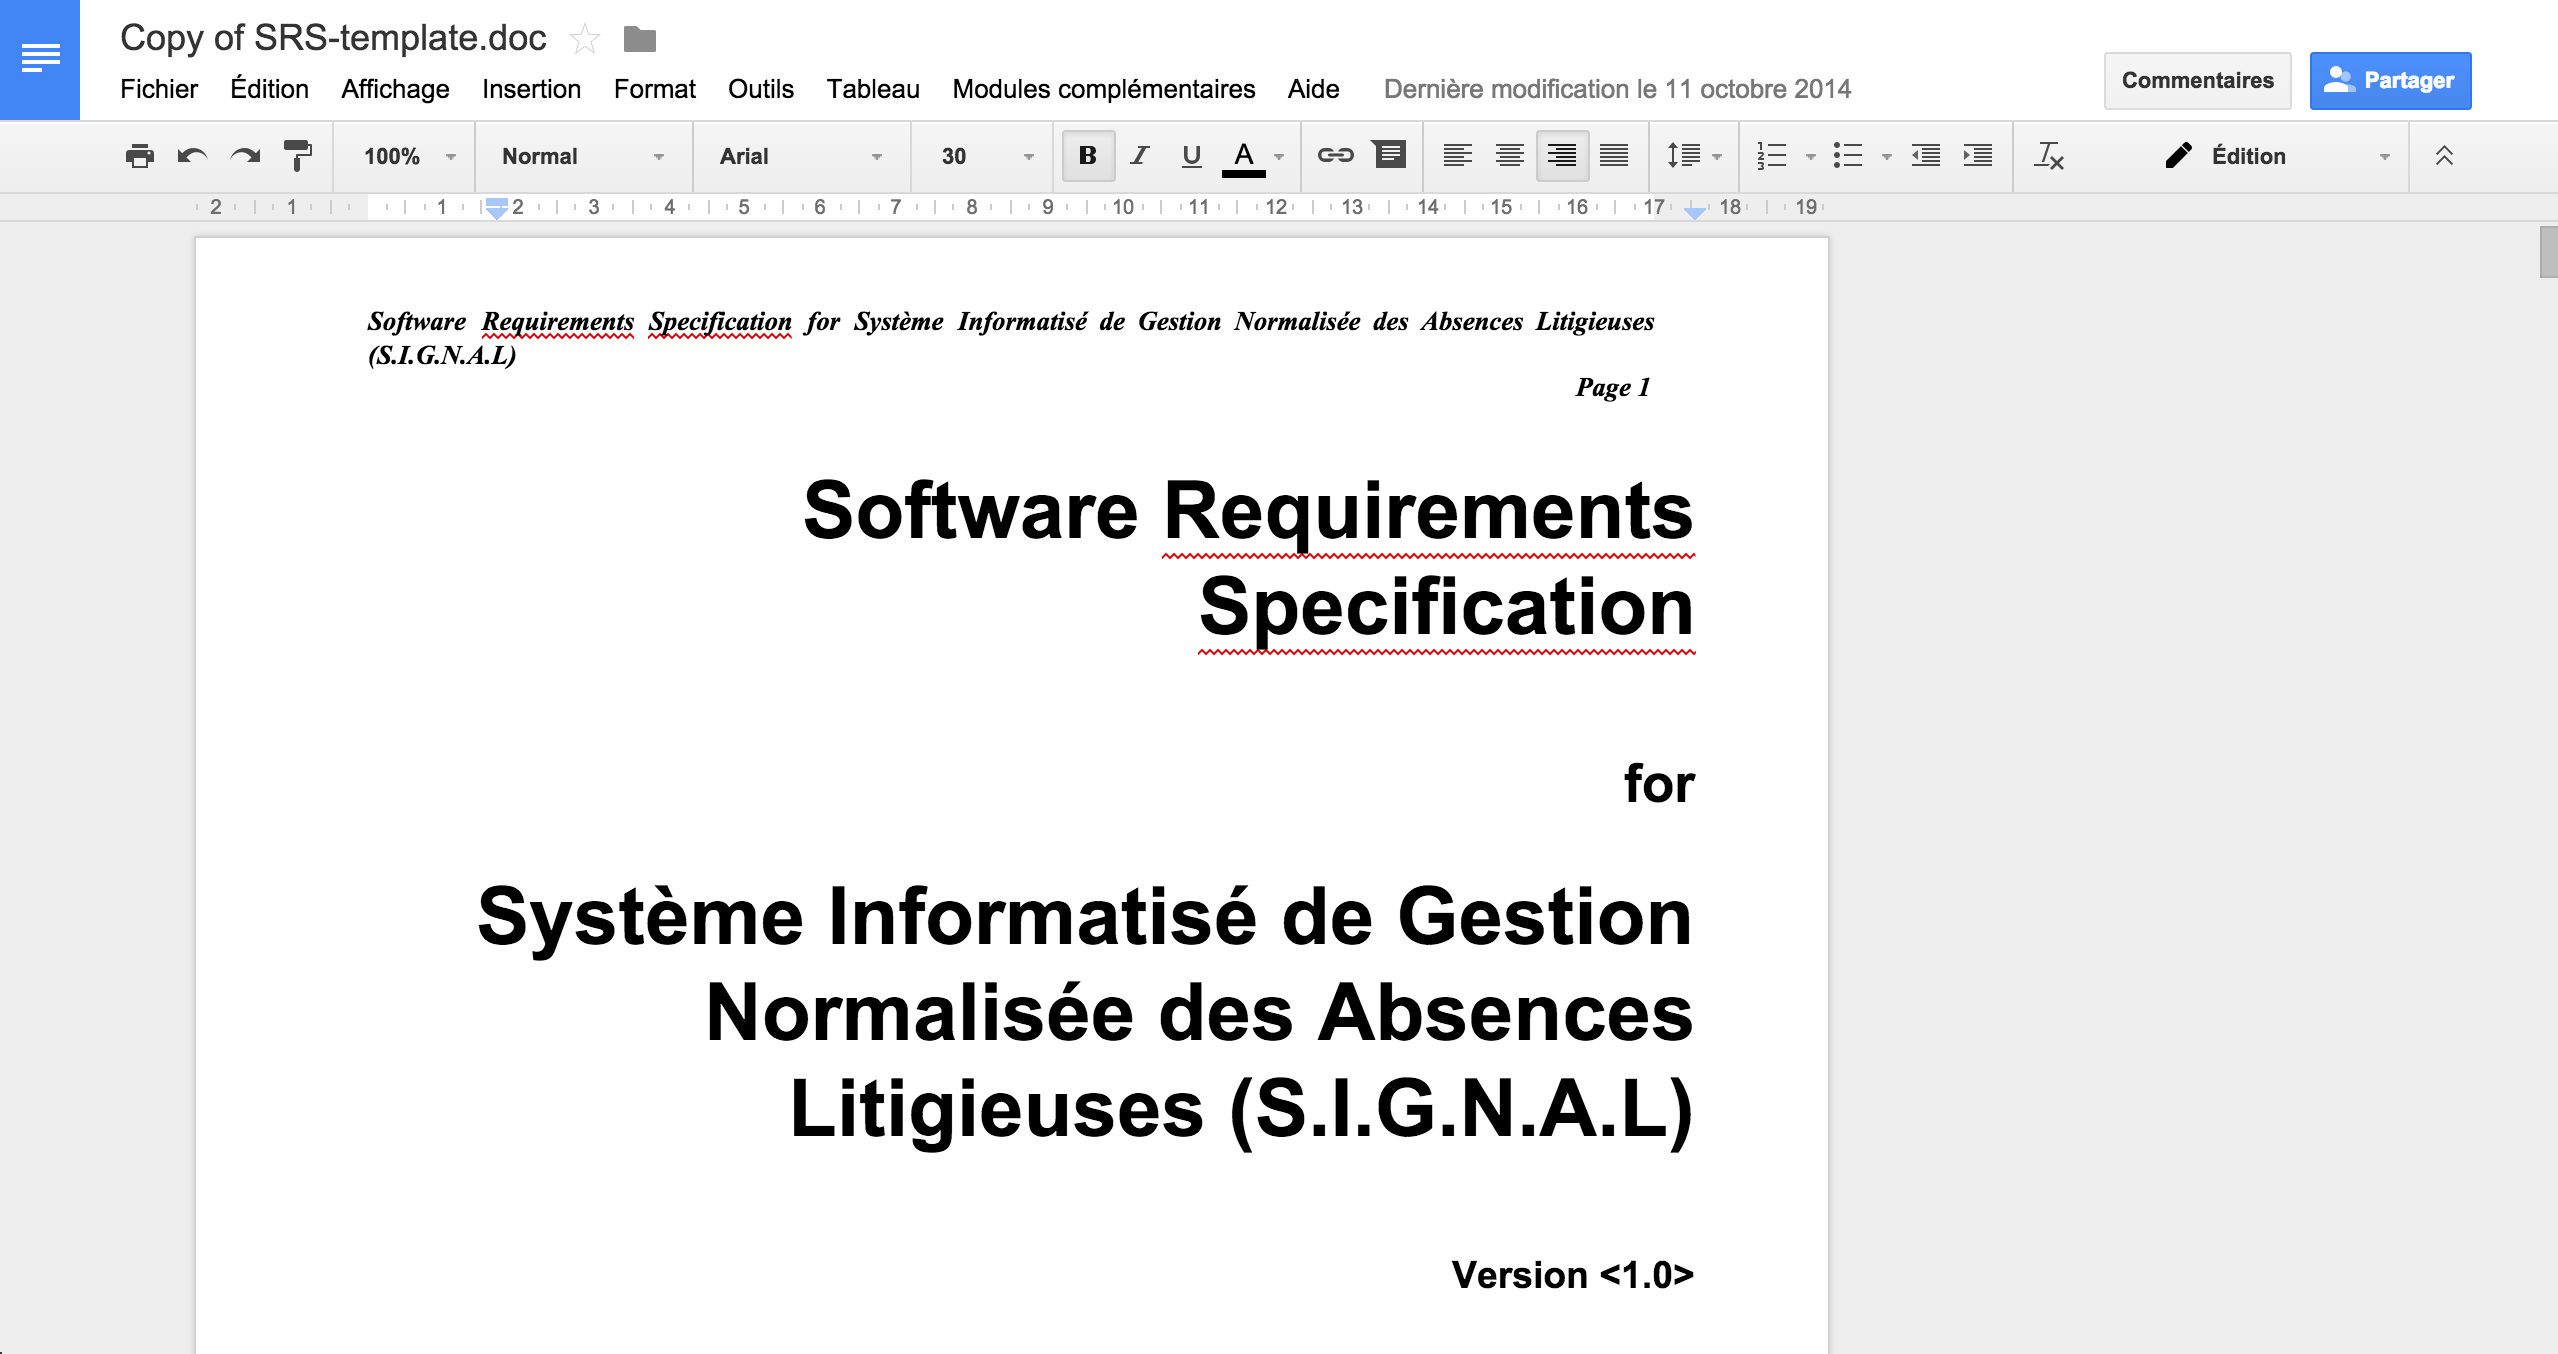
\includegraphics[width=15cm]{figures/gdoc}
  \caption{Interface de l'application Google Doc}
  \label{fig:g-doc}
\end{figure}

Toutes ces applications ont permis de rendre accessible le travail collaboratif. La présence physique de tous les contributeurs dans 
un même lieu n'est alors plus requise. Le travail sur des projets interdisciplinaires s'en trouve alors plus aisé. Chaque contributeur 
au projet peut ainsi composer tout en visualisant en temps réel la contribution des autres protagonistes. Cet aspect temps réel est 
primordial dans le domaine de l'édition collaborative, sans cela les différents contributeurs du projet ne peuvent constater 
l'évolution immédiate du document. Ce qui pourrait conduire à d'importantes erreurs dans la réalisation de ce dernier. L'application se doit donc d'être réactive pour répercuter le plus rapidement possible les différentes modifications du document. Se pose ainsi le 
problème du passage à l'échelle : si l'application offre des temps de réaction satisfaisants pour un nombre réduit de collaborateurs, 
en est-il de même pour un nombre plus important ? 

L'architecture client/serveur très largement utilisée pour ce type d'application peut montrer certaines faiblesses en période de 
montée en charge. En effet, le serveur devant gérer les communications entre tous les clients et maintenir une copie cohérente du 
document peut se retrouver débordé si le nombre de collaborateurs augmente de manière importante. Les performances de l'application se 
verraient alors dégradées, et l'expérience utilisateur entachée par des temps de latence importants. Un des moyens de répondre à cette 
problématique est de développer un réseau pair-à-pair entre tous les clients d'un même document. Les données ne transiteraient plus 
par le serveur, mais seraient directement émises d'un client vers les autres clients. Cette communication directe entre chaque client 
permet de conserver des performances correctes même en cas de montée en charge. 

J'ai ainsi pour mission d'adapter un éditeur de texte collaboratif nommé MUTE\footnote{Pour : Multi-User Text Editor, l'acronyme MUTE sera utilisé tout au long du rapport}, de façon à y incorporer un mécanisme d'échange pair-à-pair. Je dois pour cela utiliser la technologie webRTC, qui permet d'établir des connexions pair-à-pair entre deux clients par le biais du navigateur web. Mon travail consiste donc à choisir les outils de développement les 
plus adaptés pour utiliser la technologie webRTC et de développer un module de communication pair-à-pair pour l'application MUTE. 


\cleardoublepage

\chapter{Présentation de l'entreprise}

\section{Présentation du Loria}

J'ai effectué mon stage au sein de l'équipe COAST qui appartient au LORIA, Laboratoire Lorrain de Recherche en Informatique et ses Applications. 
Ce Laboratoire situé sur le campus scientifique de l'Université de Lorraine a été fondé en 1997, et ce, dans le but 
de mener des investigations dans le domaine de la recherche fondamentale et appliquée en sciences informatiques. 
Cette unité mixte regroupant plusieurs établissements, à savoir : l'Inria, le CNRS et l'Université de Lorraine est composée 
de 30 équipes regroupées en cinq départements.

Chaque département à sa propre thématique de recherche :

\begin{enumerate}
  \item Alogrithme, calcul, image et géométrie
  \item Méthodes Formelles
  \item Réseaux, Systèmes et Services
  \item Traitement des langues et des connaissances
  \item Systèmes complexes et intelligence artificielle
\end{enumerate}

Néanmois, pour les besoins de la recherche, il n'est pas rare que des collaborations s'établissent entre des équipes de différents départements. De plus, le Loria conserve un lien fort avec le monde de l'industrie au travers de collaborations avec des industrielles à l'échelle nationale ou internationale.

La figure~\ref{fig:orga} représente ainsi l'organisation du LORIA 

\begin{figure}[h!]
  \centering
  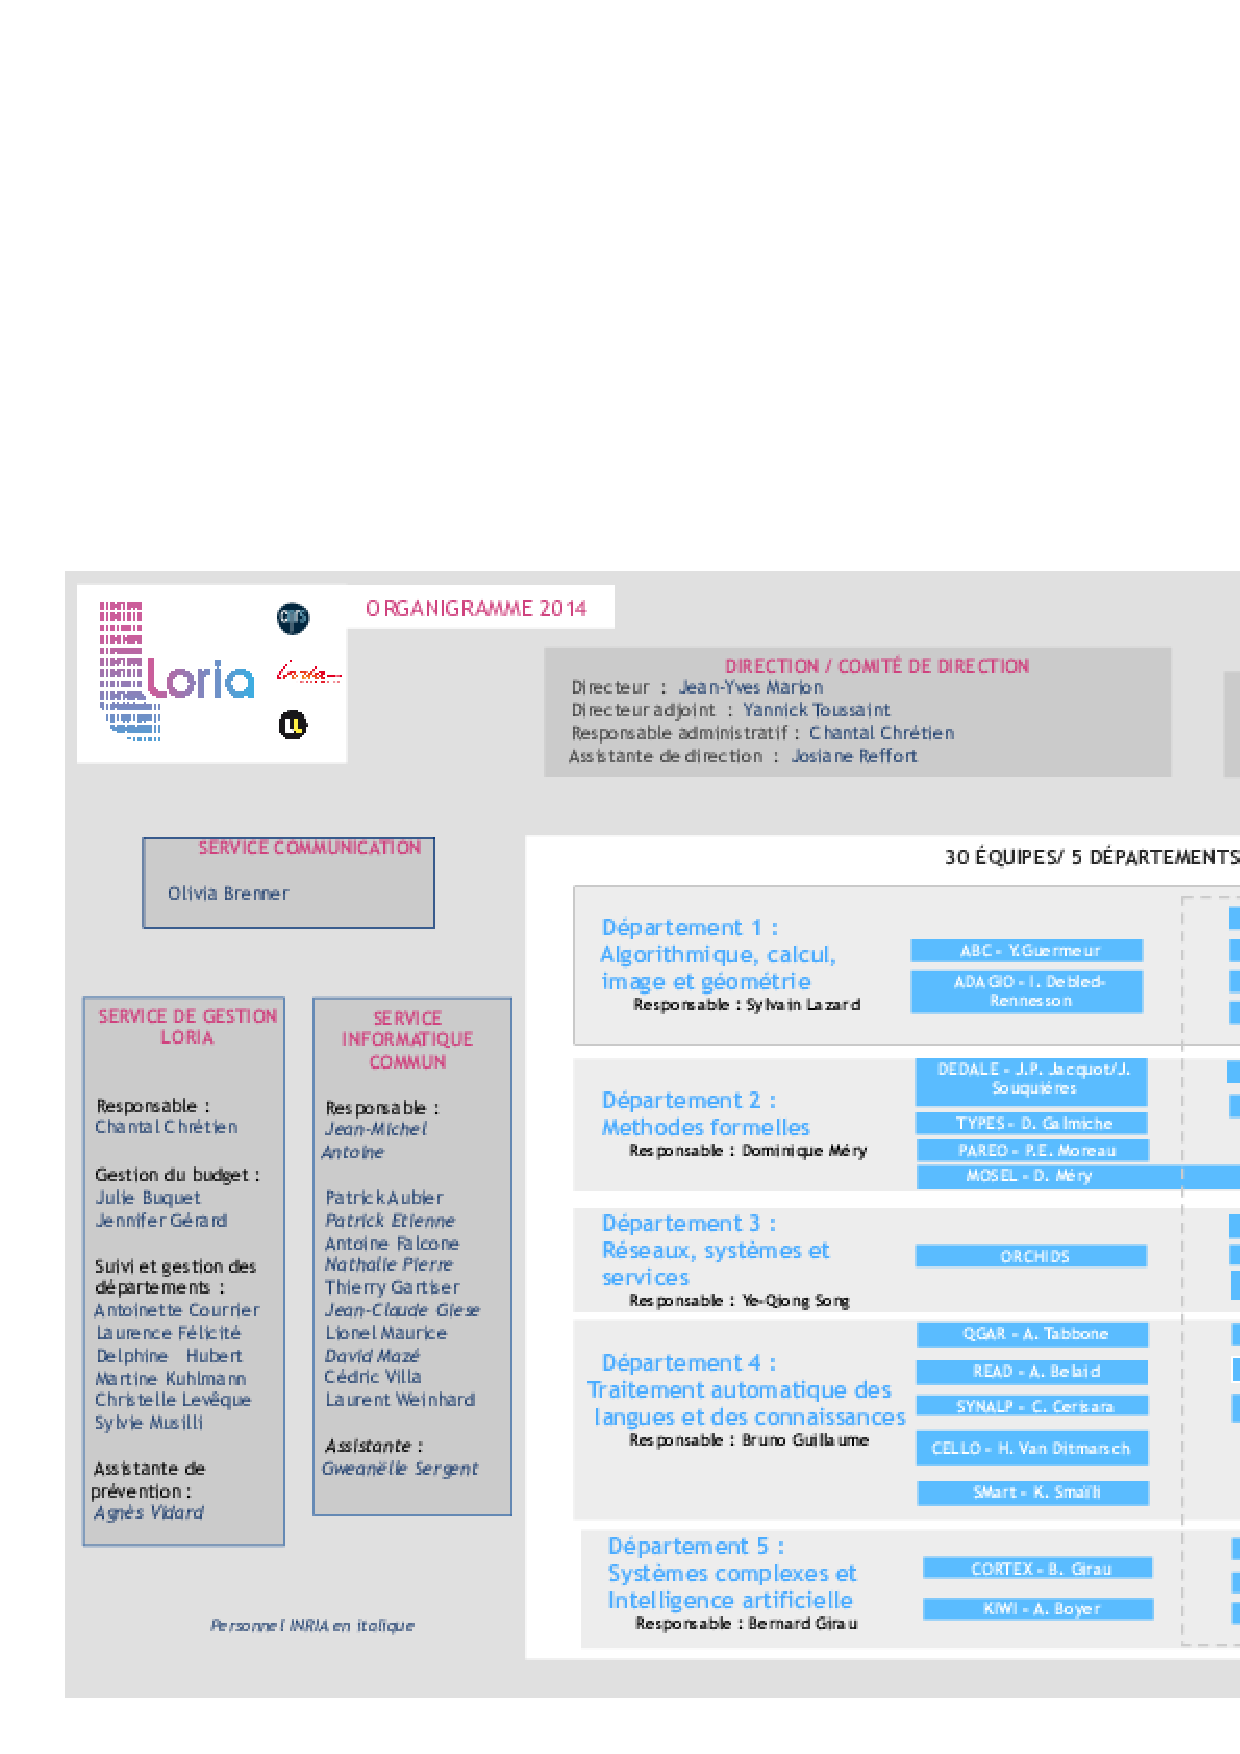
\includegraphics[width=18cm]{figures/organization}
  \caption{Organisation du Loria}
  \label{fig:orga}
\end{figure}

\section{Présentation de l'équipe COAST} 

J'ai ainsi intégré l'équipe COAST, dirigée par François CHAROY. L'équipe est composée de 23 membres, dont 11 permanents. Les recherches de cette équipe se concentrent autour du développement de services pour l'hébergement d'équipes distribuées sur internet. Ces services sont variés et s'articulent principalement autour de la co-conception et de la co-ingéieurie.

Le travail de l'équipe s'organise plus particulièrement autour de trois axes de recherche :

\begin{itemize}
  \item Systèmes collaboratifs distribués
  \item Gestion des processus "business" et service informatique
  \item Interopérabilité et modélisation d'entreprise
\end{itemize}

Mon travail au sein de l'équipe s'intégrait principalement dans le domaine des systèmes collaboratifs distribués. J'ai travaillé sous la tutelle de Gerald OSTER, enseignant chercheur au LORIA et à TELECOM Nancy. Ses recherches portent sur la réplication optimiste et cohérente dans les environnements distribués collaboratifs. Par ailleurs, j'ai travaillé en collaboration avec Mathieu NICOLAS, ingénieur de recherche dans l'équipe VERIDIS, qui a développé l'éditeur collaboratif sur lequel j'ai été amené à travailler.  

\cleardoublepage


\chapter{Etat de l'art}

\section{Présentation de MUTE}

L'application MUTE est un éditeur de texte collaboratif développé par Matthieu NICOLAS dans le cadre de la thèse de Luc ANDRÉ. La Figure~\ref{fig:screen-mute} représente l'interface proposée par l'application. Il se démarque des autres éditeurs par l'algorithme employé pour le traitement des opérations texte\footnote{Une opération texte correspond à l'ajout ou la suppression d'un caractère dans le document}. En effet, il existe deux grandes familles d'algorithme d'édition collaborative adoptant chacune une approche différente. 

L'approche la plus commune se nomme l'approche OT\footnote{Signifiant : Transformée Opérationnelles}, elle est employée dans de nombreux éditeurs de texte collaboratif, le plus connu étant Google Doc. Pour gérer les opérations concurrentes, l'algorithme utilise la transformée opérationnelle, qui résout les conflits en transformant une opération en fonction des autres opérations concurrentes. Cette méthode est relativement couteuse et n'est pas adaptée à la solution pair-à-pair choisie. 

Une seconde approche plus appropriée consiste à introduire une nouvelle structure de données permettant l'application des opérations texte concurrentes de façons désordonnées. L'ordre d'arrivée des opérations n'a donc plus d'importance dans la résolution des conflits. Cette approche se nomme approche CRDT, pour Conflict-free Replicated Data Type. L’application MUTE utilise l'algorithme LogootSplit qui est issu de cette famille. Il a été proposé par Luc ANDRÉ dans le cadre de sa thèse.

\begin{figure}[!h]
  \centering
  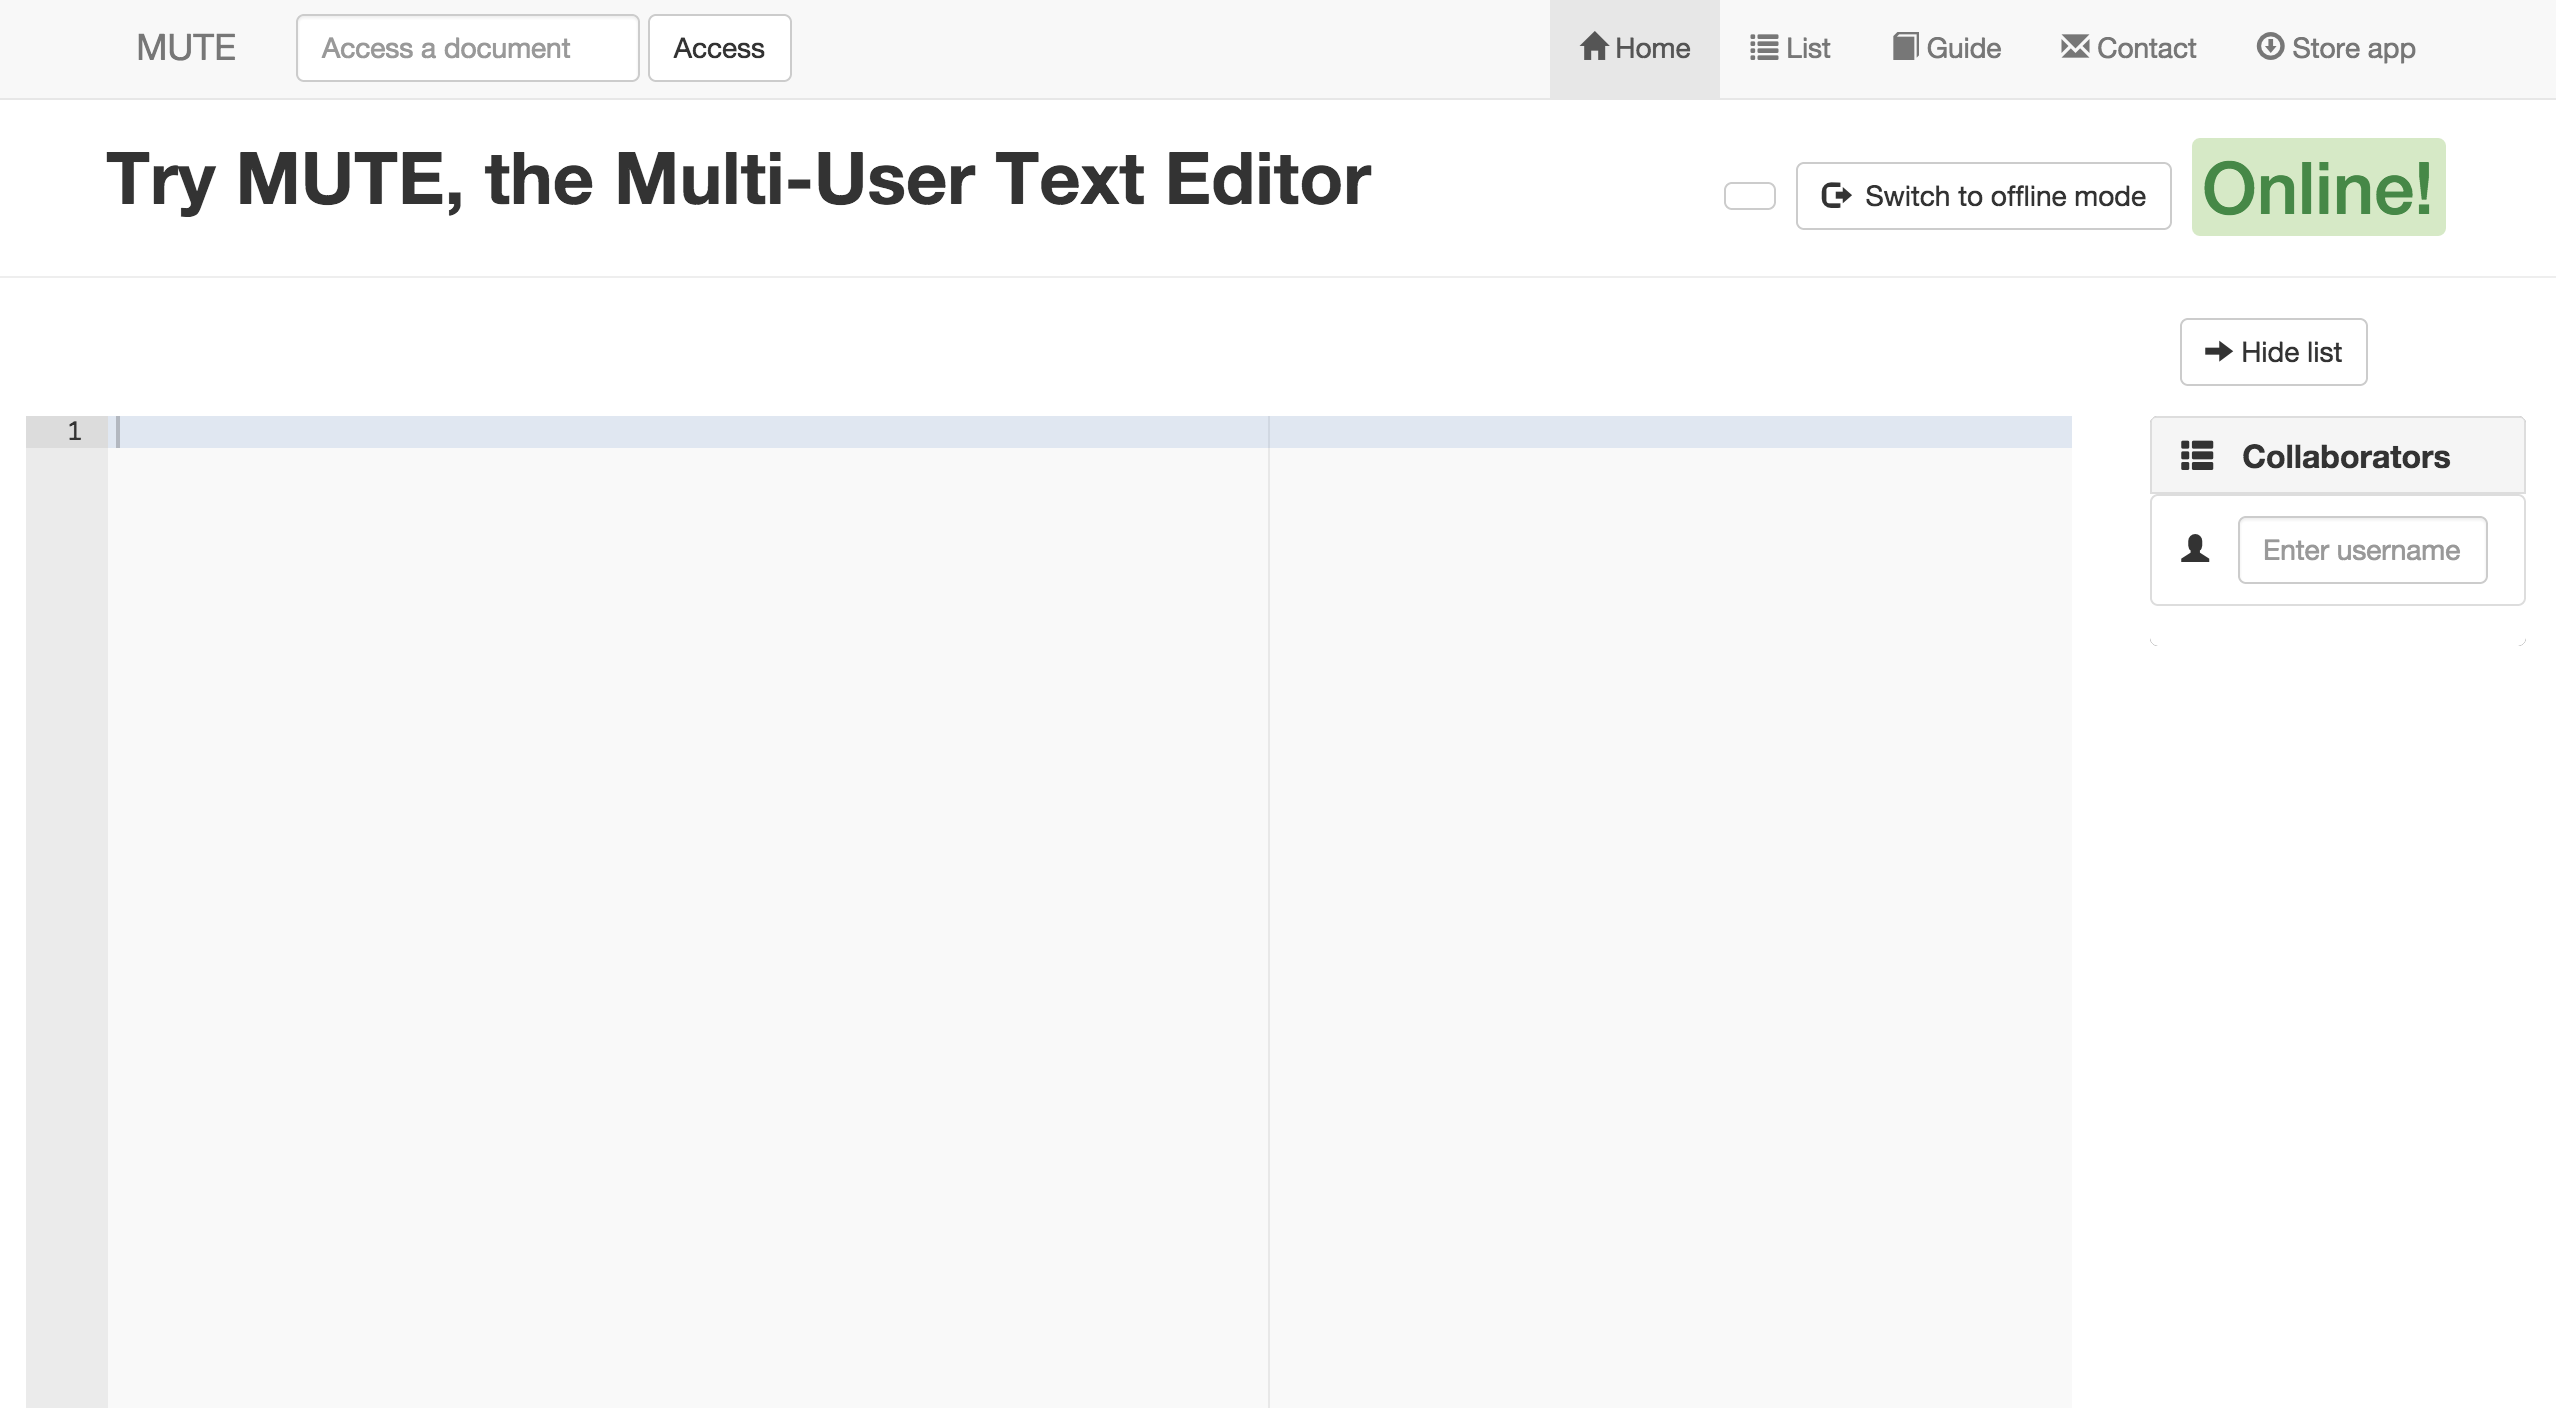
\includegraphics[width=14cm]{figures/screenshot-mute}
  \caption{Interface de l'application MUTE}
  \label{fig:screen-mute}
\end{figure}


\subsection{Architecture et fonctionnement de MUTE}

L'application MUTE adopte initialement une architecture client/serveur. Tous les collaborateurs d'un même document sont connectés à un serveur qui se charge de relayer les différentes opérations texte et de maintenir une copie du document. Chaque client possède une copie du document ainsi que des informations relatives à l'utilisateur, comme son nom et la position de son curseur. Il possède également ces informations pour les autres collaborateurs du document. Tous les clients sont connectés au serveur au travers d'une webSocket\footnote{Connexion client/serveur persistante}. Comme le montre la Figure~\ref{fig:cli-serv}, le serveur est l'élément central de toutes les communications. Il conserve une trace de tous les documents et associe à chaque document les contributeurs de ce dernier et une copie du document. De cette façon, lorsqu'un nouveau client se connecte, ce dernier a la possibilité de récupérer la dernière copie du document en cours d'édition. 

\begin{figure}[!h]
  \centering
  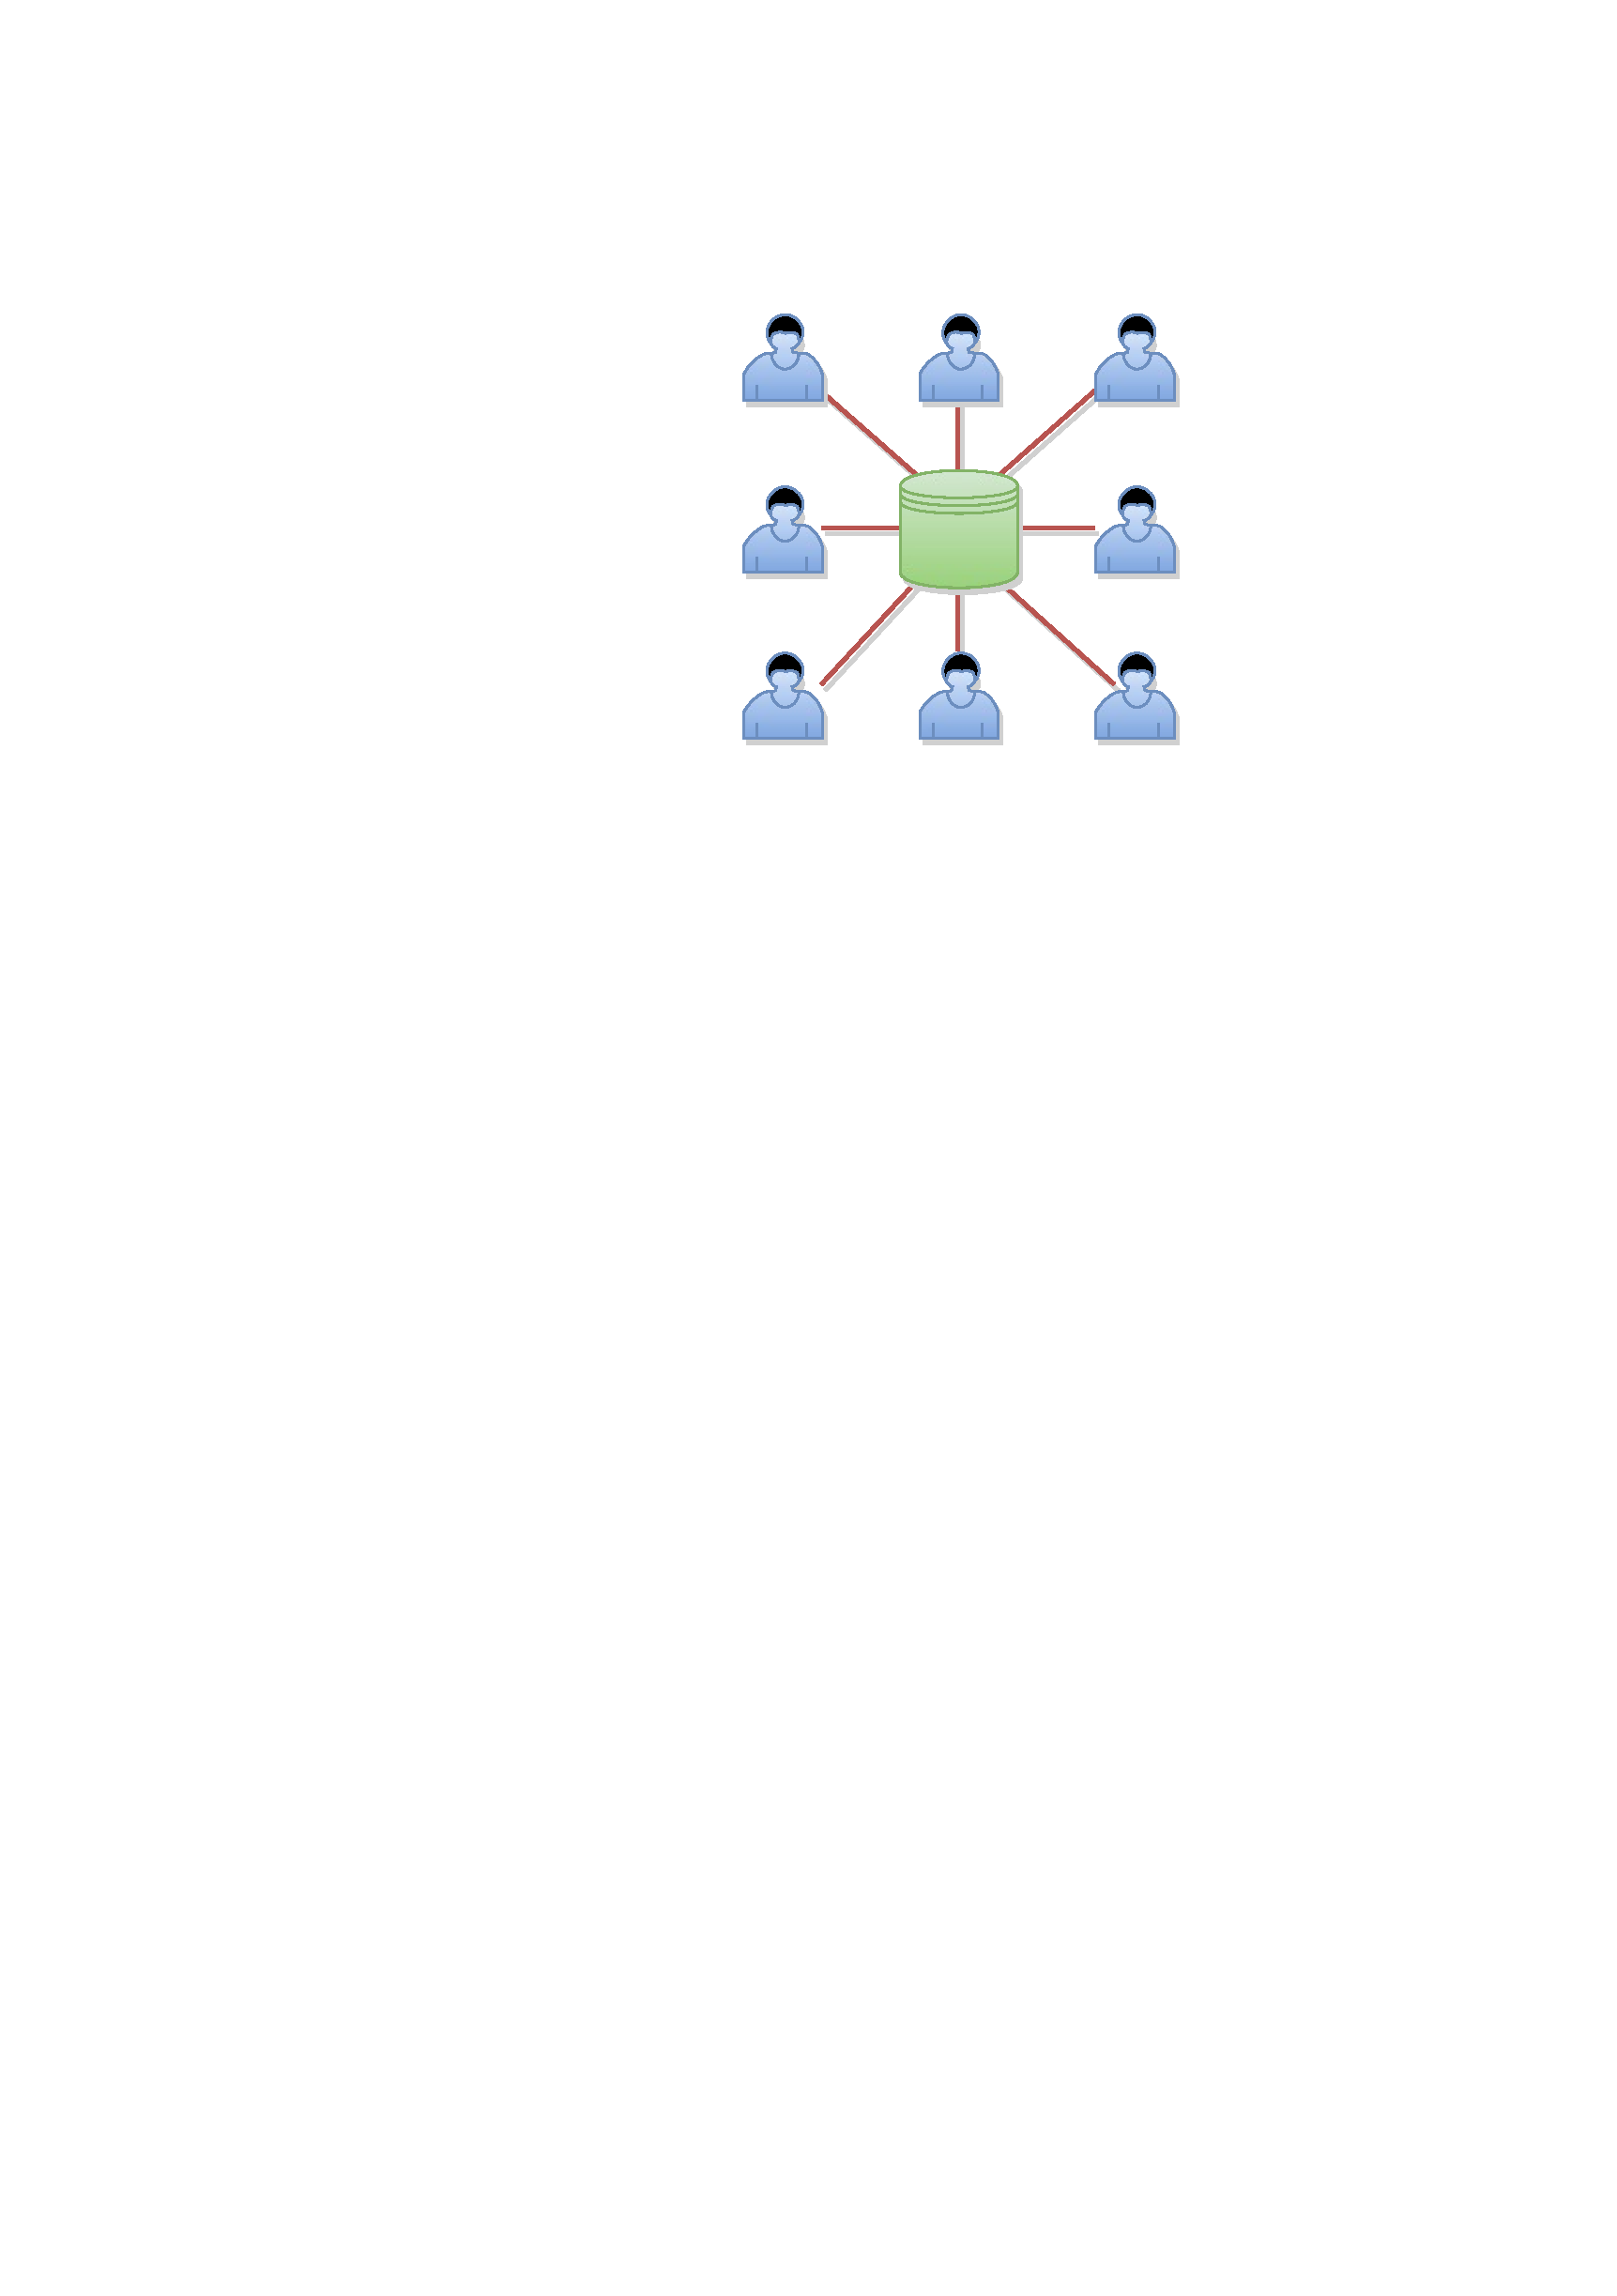
\includegraphics[width=5cm]{figures/client-server}
  \caption{Architecture client/serveur - le serveur au centre de toutes les communications}
  \label{fig:cli-serv}
\end{figure}



\subsubsection{Architecture du client}
Le client est composé de quatre modules :

\begin{itemize}
    \item Ace-editor\footnote{Pour plus d'information : \url{http://ace.c9.io/}} : librairie utilisée pour créer l'éditeur de texte qui apparait à l'écran du client
    \item InfoUser : module permettant de gérer les informations de l'utilisateur et des autres contributeurs
    \item Coordinator : module permettant de gérer le modèle \footnote{Sous la forme de structures LogootSplit} et utilisant l'algorithme LogootSplit pour l'application des opérations texte
    \item Socket-io-adapter : module en charge de la communication avec le serveur
\end{itemize}

L'organisation de ces modules est décrite dans la Figure~\ref{fig:mute-archi} 
Chaque collaborateur est identifié de manière unique grâce à un \emph{numéro de site} attribué par le serveur. 

\subsubsection{Architecture du serveur}
L'architecture du serveur décrite par la Figure~\ref{fig:mute-archi} est semblable à celle du client, à la différence qu'elle n'utilise pas Ace-editor.
Elle se compose donc de trois modules :

\begin{itemize}
  \item InfoUser : module permettant de gérer les informations de tous les utilisateurs d'un document
  \item Coordinator : module permettant de gérer le modèle et utilisant l'algorithme LogootSplit pour l'application des opérations texte
  \item Socket-io-adapter : module en charge de la communication avec les clients
\end{itemize}


\subsubsection{Fonctionnement de MUTE}

La Figure~\ref{fig:mute-archi} représente le fonctionnement de l'architecture MUTE. Deux clients et le serveur y sont représentés, un client est en train de rédiger, pendant que le second visualise les modifications. Le cheminement des données est représenté par des flèches et chaque étape est décrite dans les encadrés bleus.

Lorsqu'un client écrit dans l'éditeur, le module Ace-editor génère des opérations texte qui vont être transmises au coordinateur\footnote{Ou coordinator en anglais}. Le coordinateur va en suite générer les opérations Logoot pour les opérateurs distants\footnote{Les opérateurs distants correspondent aux autres clients et au serveur} et va transmettre ces opérations au module socket-io-adapter. Les opérations vont être ainsi transmises au serveur.

À la réception des opérations Logoot par le serveur, ce dernier va transmettre ces opérations à son coordinateur et dans le même temps, les enverra aux autres contributeurs du document. Le coordinateur du serveur va appliquer les opérations Logoot de façon à conserver une copie à jour du document. Les autres contributeurs vont faire de même et vont répercuter les modifications sur leur modèle local. Une fois les opérations appliquées, la vue de l'éditeur va se mettre à jour pour que les autres utilisateurs puissent visualiser les modifications.

\begin{figure}[!h]
  \centering
  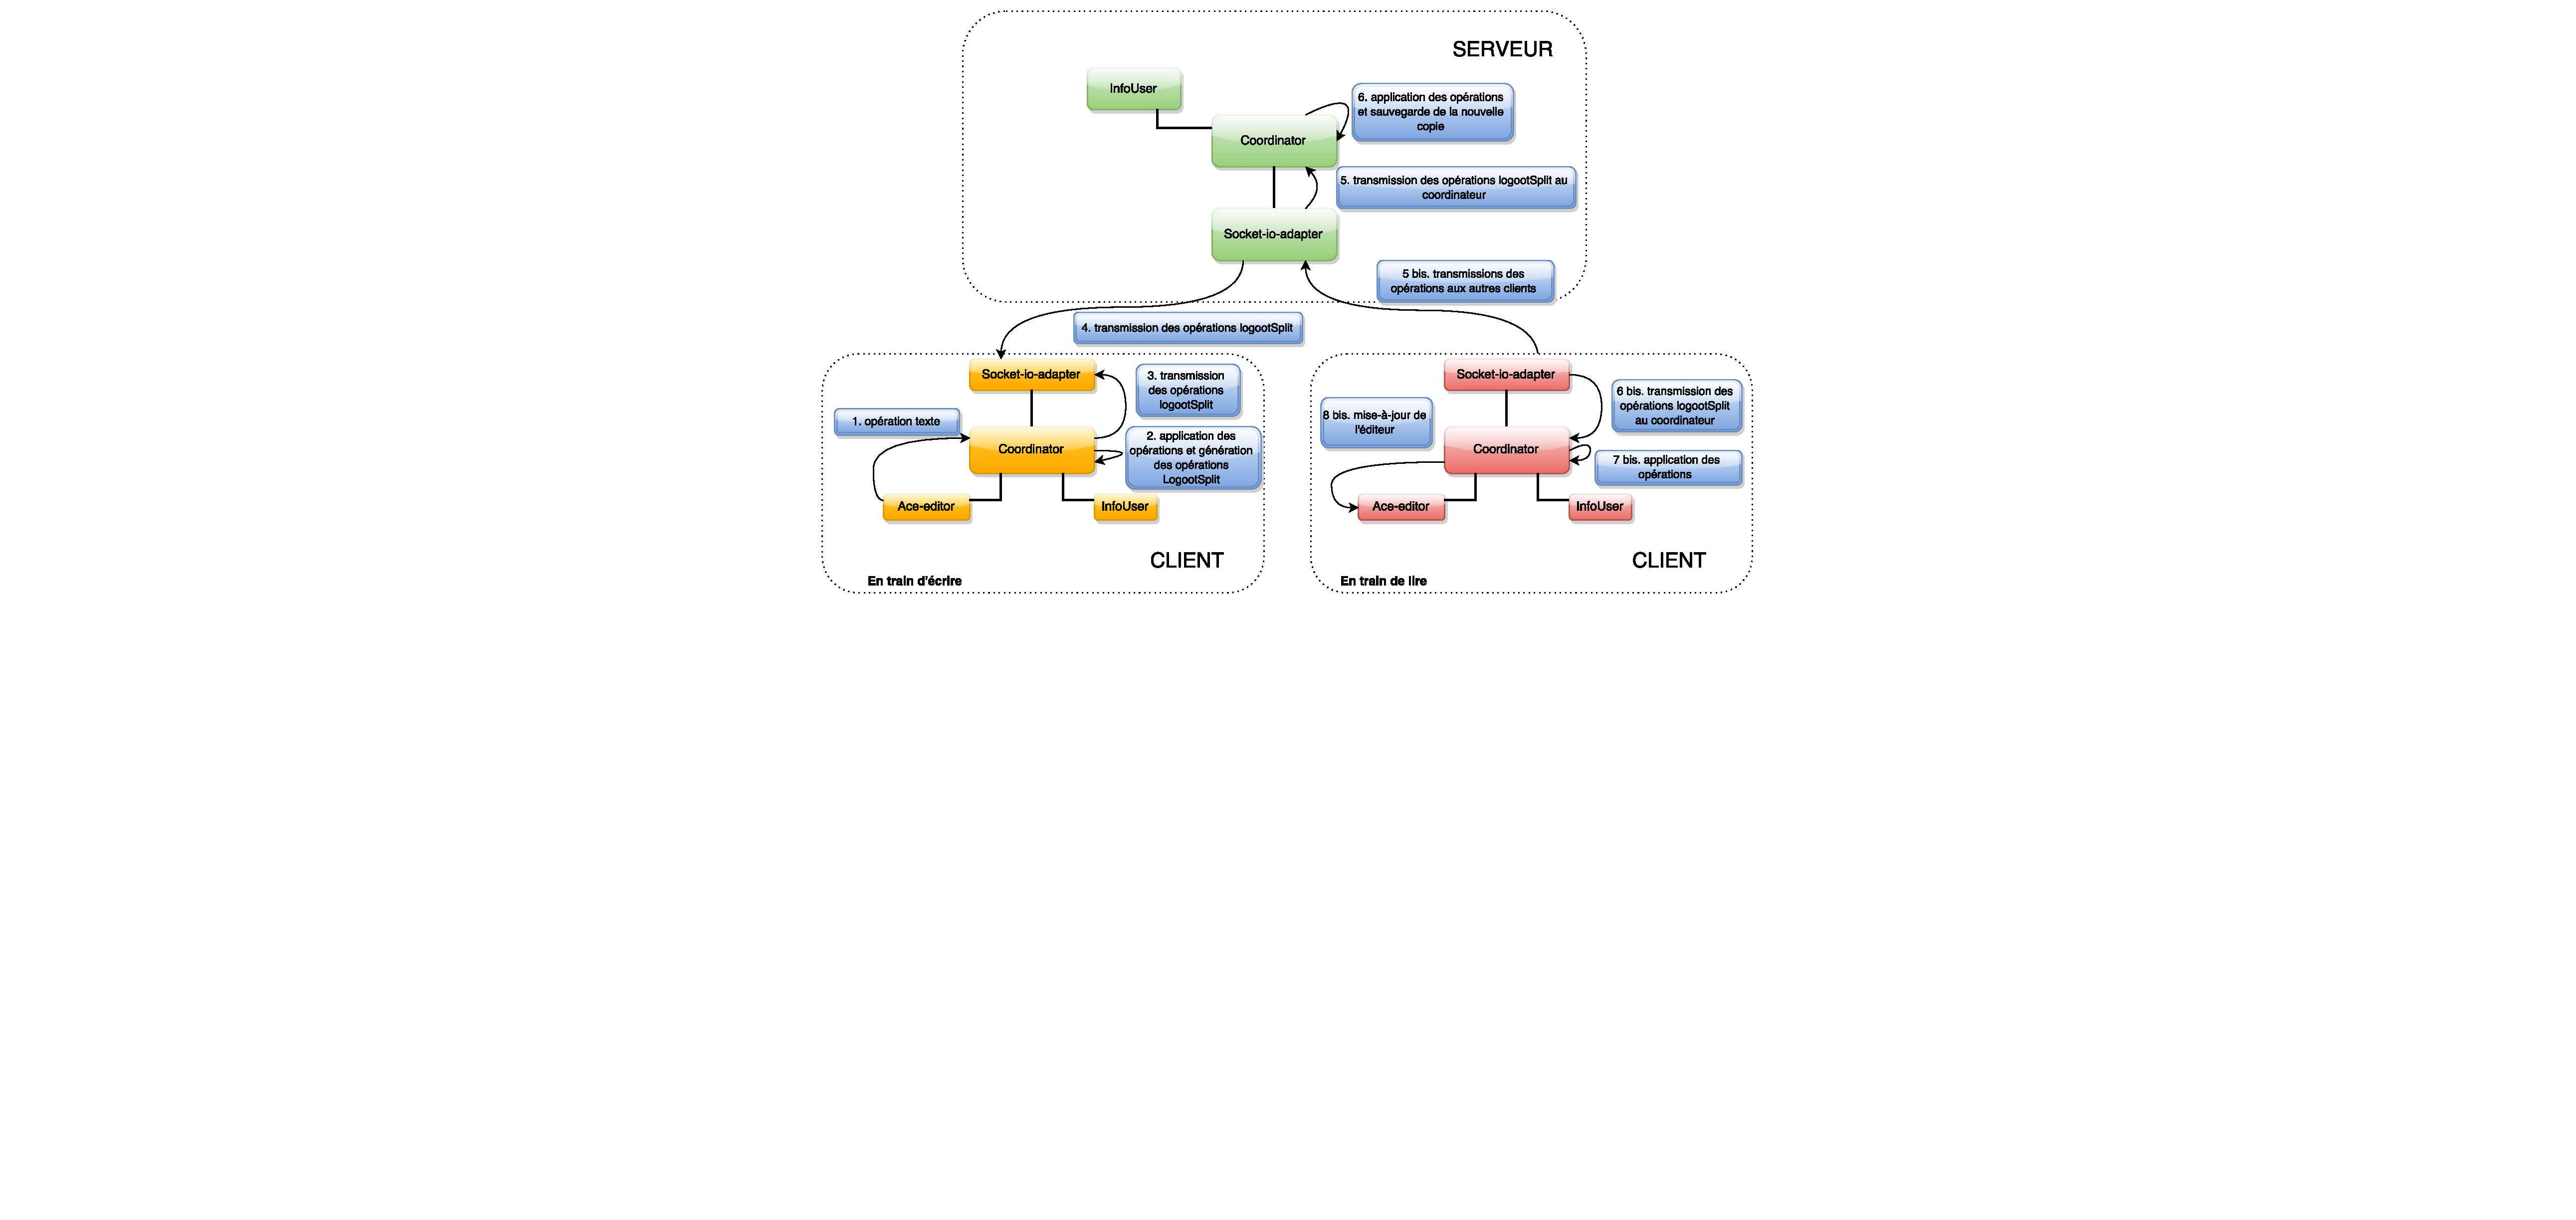
\includegraphics[width=17cm]{figures/MUTE-archi}
  \caption{Architecture et fonctionnement de l'application MUTE}
  \label{fig:mute-archi}
\end{figure}

\subsubsection{Avantages et limites de cette architecture}

Cette architecture est adaptée pour le développement rapide d'un prototype fonctionnel. Elle permet une gestion centralisée des documents et les nombreuses librairies disponibles permettent de gérer de façon fiable les connexions client-serveur. Cependant cette architecture rencontre des problèmes de passage à l'échelle. En effet, le serveur devant gérer l'ensemble des documents et toutes les communications avec les clients peut se retrouver rapidement débordé si le nombre de documents et/ou de collaborateurs venait à augmenter. Une solution pourrait être d'augmenter les moyens matériels, à savoir la puissance des serveurs, cependant cette solution est relativement couteuse et non viable sur le long terme.

Il est alors nécessaire de s'affranchir de cette architecture centralisée du moins pour les échanges d'opérations texte, de façon à soulager le serveur. Une solution est donc de créer des connexions directes entre les clients. Une technologie nommée webRTC permet de créer des connexions pair-à-pair entre clients par le biais d'un navigateur web. Cette solution a été retenue pour répondre au problème de scalabilité du système.


%La Figure~\ref{fig:logo-tn} représente le logo de \reportSchool{}.%

% Ceci est une référence bibliographique~\cite{GOT4}.

\section{Présentation des technologies webRTC}
WebRTC pour \emph{Real Time Communication} est un standard de communication élaboré par le W3C \footnote{RFC de webRTC : \url{http://www.w3.org/TR/webrtc/}}. Ce standard encore à l'étude aujourd'hui a été initié en mai 2011 et a pour principal objectif de permettre la communication en temps réel de différents médias\footnote{À savoir : vidéo, audio et tout autre type de données}. WebRTC doit donc permettre d'établir une connexion pair-à-pair entre deux clients web, mais doit également permettre la gestion des flux de données. 

Pour ce faire, webRTC propose l'implémentation de trois APIs JavaScript :
\begin{itemize}
  \item MediaStream : En charge de synchroniser les flux de données pouvant par exemple provenir de la webcam ou du micro de l'ordinateur
  \item RTCPeerConnection : En charge de gérer la bande passante et le chiffrement des données
  \item RTCDataChannel : En charge de gérer la connexion pair-à-pair entre deux clients\\
\end{itemize}

Tous les navigateurs n'implémentent pas encore ces APIs, la technologie webRTC est principalement disponible sur les dernières versions de :
\begin{itemize}
  \item Mozilla Firefox
  \item Google Chrome
  \item Opera
  \item Android Browser et Chrome for Android\\
\end{itemize}

En somme, grâce à ces APIs, il est possible d'utiliser les flux de données provenant de la webcam ou du micro et de le diffuser via une connexion pair-à-pair à d'autres clients. Cette technologie a permis le développement de nombreuses applications de messagerie instantanée et de visioconférence. Le dernier exemple connu se nomme Firefox Hello\footnote{Pour plus d'information : \url{https://www.mozilla.org/fr/firefox/hello/}}.

\subsection{Les mécanismes réseau utilisés}

Outre la gestion des flux de média, certains mécanismes ont été introduits au niveau du réseau permettant l'établissement d'une connexion pair-à-pair entre deux clients distants, ainsi que la résolution de certaines difficultés induites par les pare-feu\footnote{Ou firewall en anglais} et par les NAT\footnote{Signifiant : Network Address Translation}.

\subsubsection{Serveur de signaling}

Une des premières difficultés à laquelle il est nécessaire de répondre est l'établissement d'une connexion pair à paire entre deux clients distants. Il est en effet nécessaire d'avoir un mécanisme de contrôle permettant d'initialiser la connexion, d'échanger les IPs et les ports applicatifs de chaque machine et d'assurer que les deux clients soient bien compatibles. Un serveur de signaling se charge donc de l'échange de ces différents messages de contrôle. 

Ainsi, quand un client souhaite entamer une connexion pair-à-pair avec un autre client, il va tout d'abord contacter le serveur de signaling. Une fois le second client disposé à recevoir la demande, le serveur va la lui transmettre. Une succession d'échange va alors s'effectuer pour que la connexion pair-à-pair puisse s'établir correctement. 

Trois types d'information sont échangés par l'intermédiaire du serveur de signaling :
\begin{itemize}
    \item Des messages de contrôle, pour l'initialisation de la connexion et la gestion des erreurs
    \item Des messages liés à la configuration du réseau\footnote{Adressage IP et numéro de port}
    \item Des messages liés à la compatibilité des médias\footnote{Codecs vidéo et résolution}\\
\end{itemize}

Une fois ces différentes informations échangées et la compatibilité assurée, la connexion pair-à-pair peut être établie comme le montre la Figure~\ref{fig:signaling}

\begin{figure}[!h]
  \centering
  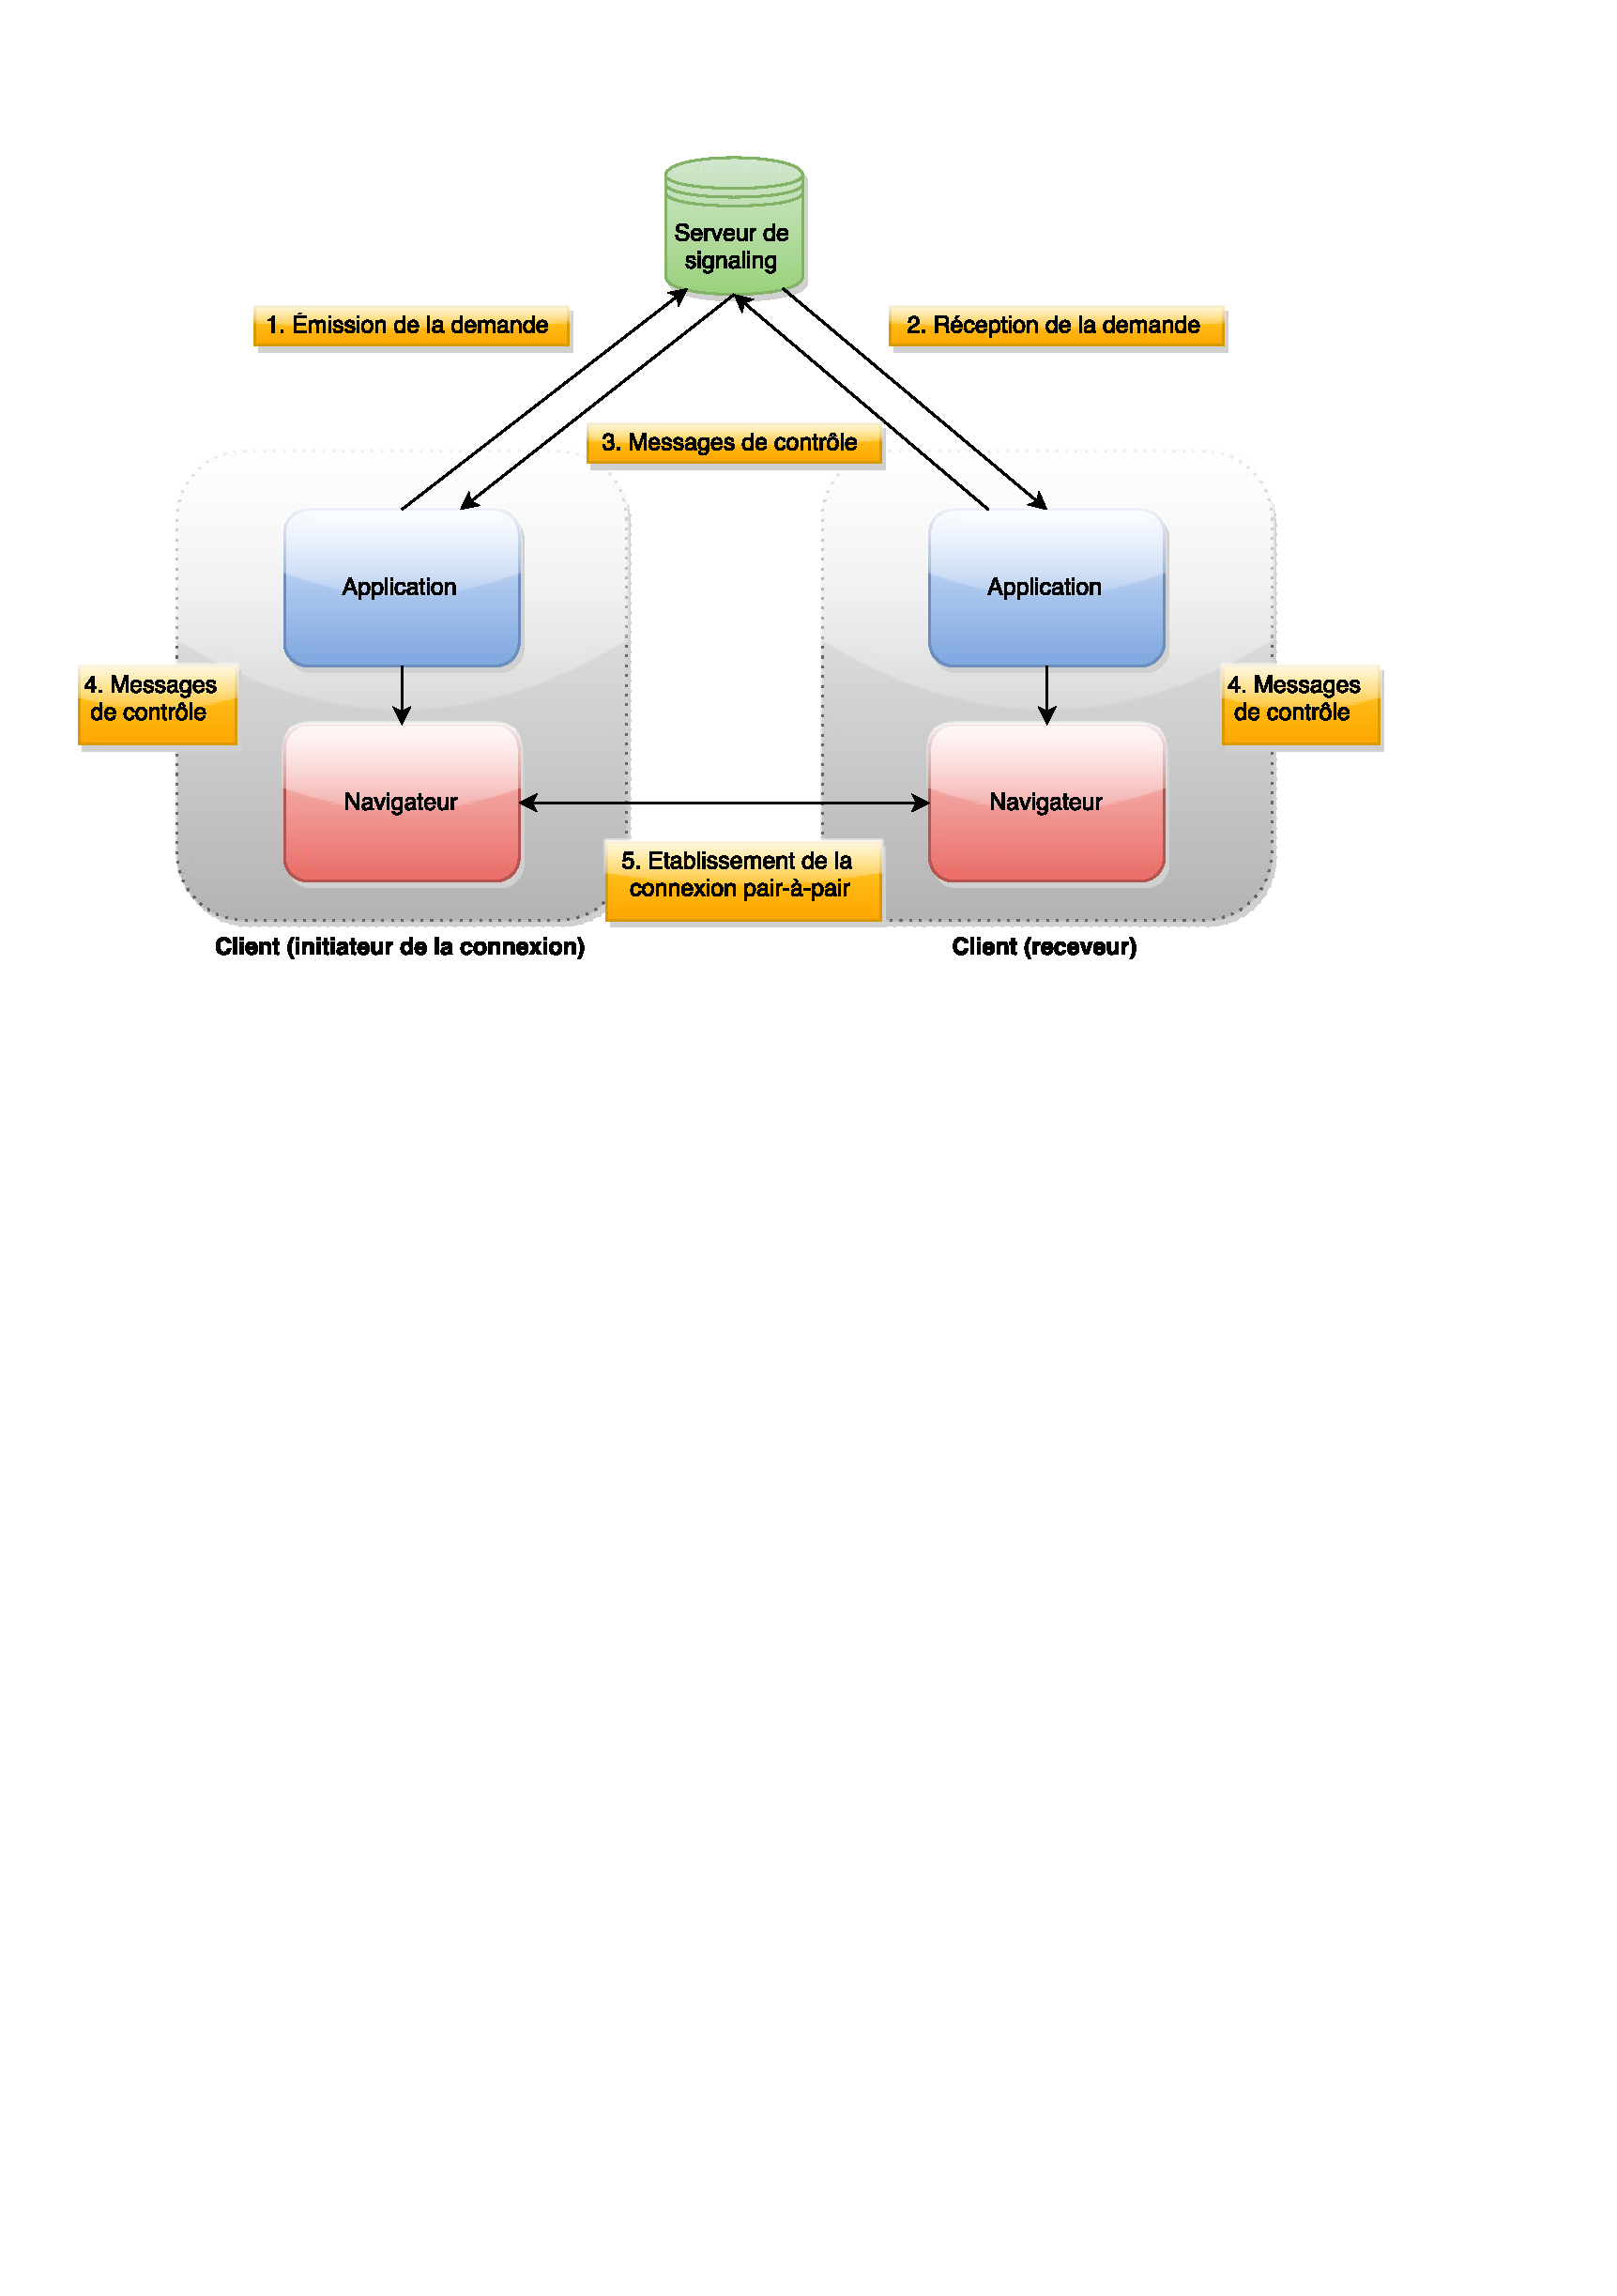
\includegraphics[width=10cm]{figures/signaling}
  \caption{Mécanisme de "signaling" pour l'initialisation d'une connexion pair-à-pair \emph{(inspiré de la référence bibliographique~\cite{GettingStartedwithWebRTC})}}
  \label{fig:signaling}
\end{figure}

Il est important de préciser que le serveur de signaling ne fait pas l'objet de spécification dans le standard webRTC. Les développeurs ne sont donc pas contraints ni dans le choix d'un protocole de communication ni dans le choix d'une technologie pour la communication client/serveur.

\subsubsection{Serveur STUN et TURN}

Pour créer une connexion pair-à-pair, il est également nécessaire d'obtenir une adresse IP publique et un numéro de port sur lequel se connecter. De nombreux éléments intermédiaires comme les NAT peuvent empêcher l'obtention de ces informations. Pour pallier à ce problème webRTC spécifie l'utilisation de serveurs STUN\footnote{Pour : Simple Traversal of UDP through NATs} utilisant le protocole ICE\footnote{Pour : Interactive Connectivity Establishement}. Ce protocole\footnote{RFC de ICE : \url{https://tools.ietf.org/html/rfc5245}} permet donc de répurérer une adresse IP publique et un numéro de port même en cas de présence de NAT.

La Figure~\ref{fig:stun} représente de cette manière la place des serveurs STUN dans le contexte d'une connexion pair-à-pair. Le nuage aux contours bleus représente le serveur de signaling qui se charge de l'échange des messages de contrôle (notamment des adresses publiques), tandis que les serveurs STUN attribuent à chaque client une adresse IP publique est un numéro de port.

\begin{figure}[!h]
  \centering
  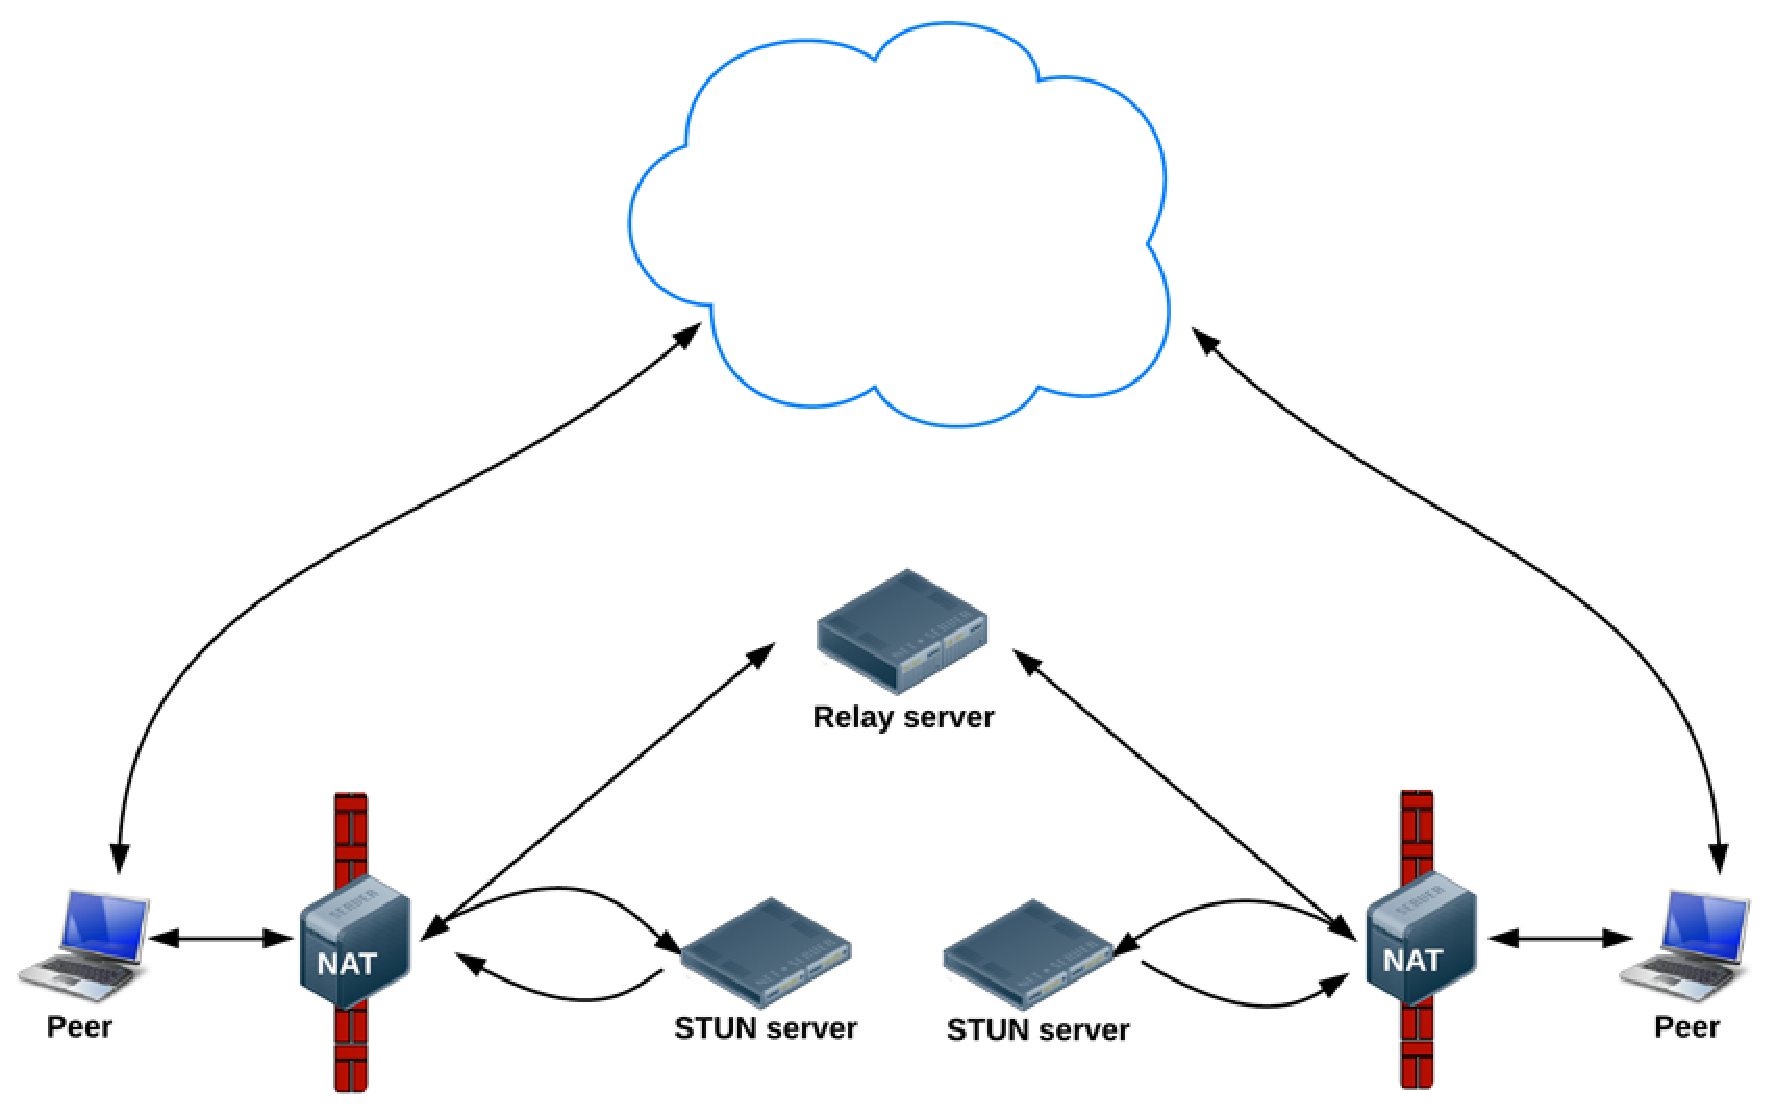
\includegraphics[width=14cm]{figures/stun}
  \caption{Établissement d'une connexion avec un serveur STUN \emph{(figure issue de la référence bibliographique~\cite{GettingStartedwithWebRTC})}}
  \label{fig:stun}
\end{figure}

Le problème d'attribution d'adresses publiques étant résolu, les pairs vont alors tenter de s'interconnecter directement. La présence d'un serveur proxy ou d'un pare-feu peut cependant poser problème et empêcher l'établissement de la connexion. Dans ce cas-là, l'information doit transiter par un serveur TURN\footnote{Pour : Traversal Using Relays around NAT}. La Figure~\ref{fig:turn} représente la place occupée par un serveur TURN dans le contexte d'une connexion pair-à-pair bloquée parla présence d'un pare-feu ou d'un serveur proxy. Les serveurs TURN jouent alors le rôle de relais.

\begin{figure}[!h]
  \centering
  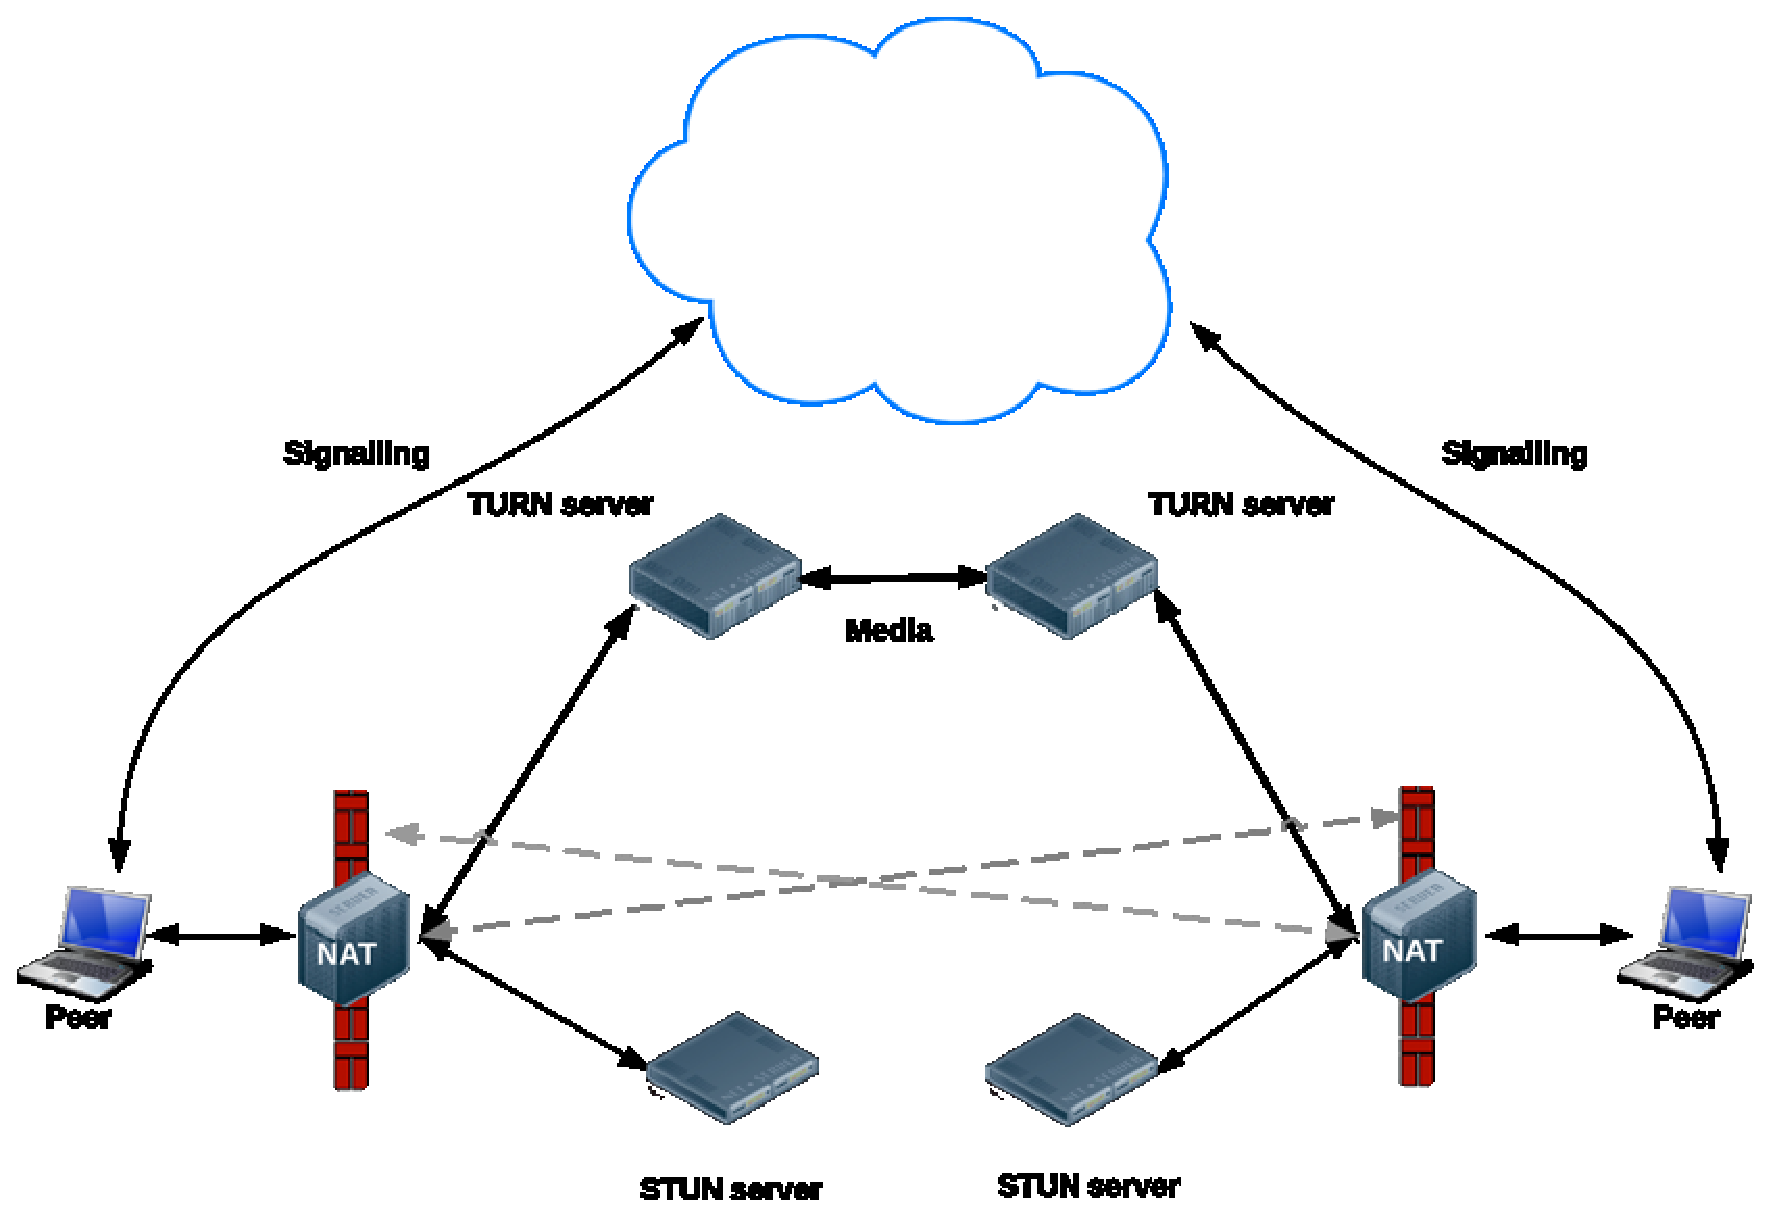
\includegraphics[width=14cm]{figures/turn}
  \caption{Fonctionnement d'un serveur TURN \emph{(figure issue de la référence bibliographique~\cite{GettingStartedwithWebRTC})}}
  \label{fig:turn}
\end{figure}

Ces différents mécanismes permettent de répondre aux contraintes imposées par internet et garantissent l'établissement d'une connexion RTC. 

\cleardoublepage

\chapter{Présentation du travail réalisée}

J'ai pour mission d'intégrer un module de communication pair-à-pair dans l'application MUTE. Mon travail consiste donc à comprendre et appréhender l'architecture de MUTE, d'étudier et de choisir la librairie la plus adaptée pour utiliser la technologie webRTC et enfin de développer un module de communication pair-à-pair opérationnel.

\section{Présentation du contexte et de la problématique détaillée}

MUTE est une application développée en JavaScript, l'application côté serveur a été développée en NodeJS, l'application côté client utilise certains modules NodeJS, mais également des librairies JavaScript externes\footnote{JQuey, Ace-editor , etc.}.

Le module de communication pair-à-pair sera intégré au même niveau que le module de communication client/serveur\footnote{Socket-io-adapter}. Les fonctionnalités initialement proposées seront conservées et l'utilisateur pourra choisir ou non d'utiliser la communication pair-à-pair. L'objectif n'est donc pas de modifier l'existant, mais d'adapter le module de communication pair-à-pair aux mécanismes déjà utilisés. Dans le cas où des modifications venaient à être effectuées sur les modules existants, elles ne devraient en rien  altérer le comportement des fonctionnalités existantes.

L'objectif est d'aboutir à une topologie identique à celle décrite à la Figure~\ref{fig:topo-webRTC}. On remarque ainsi que tous les contributeurs sont interconnectés. De plus, une connexion persistante est établie entre le serveur et les clients de façon à ce que le serveur ait connaissance des contributeurs, et ce pour chaque document.

\begin{figure}[!h]
  \centering
  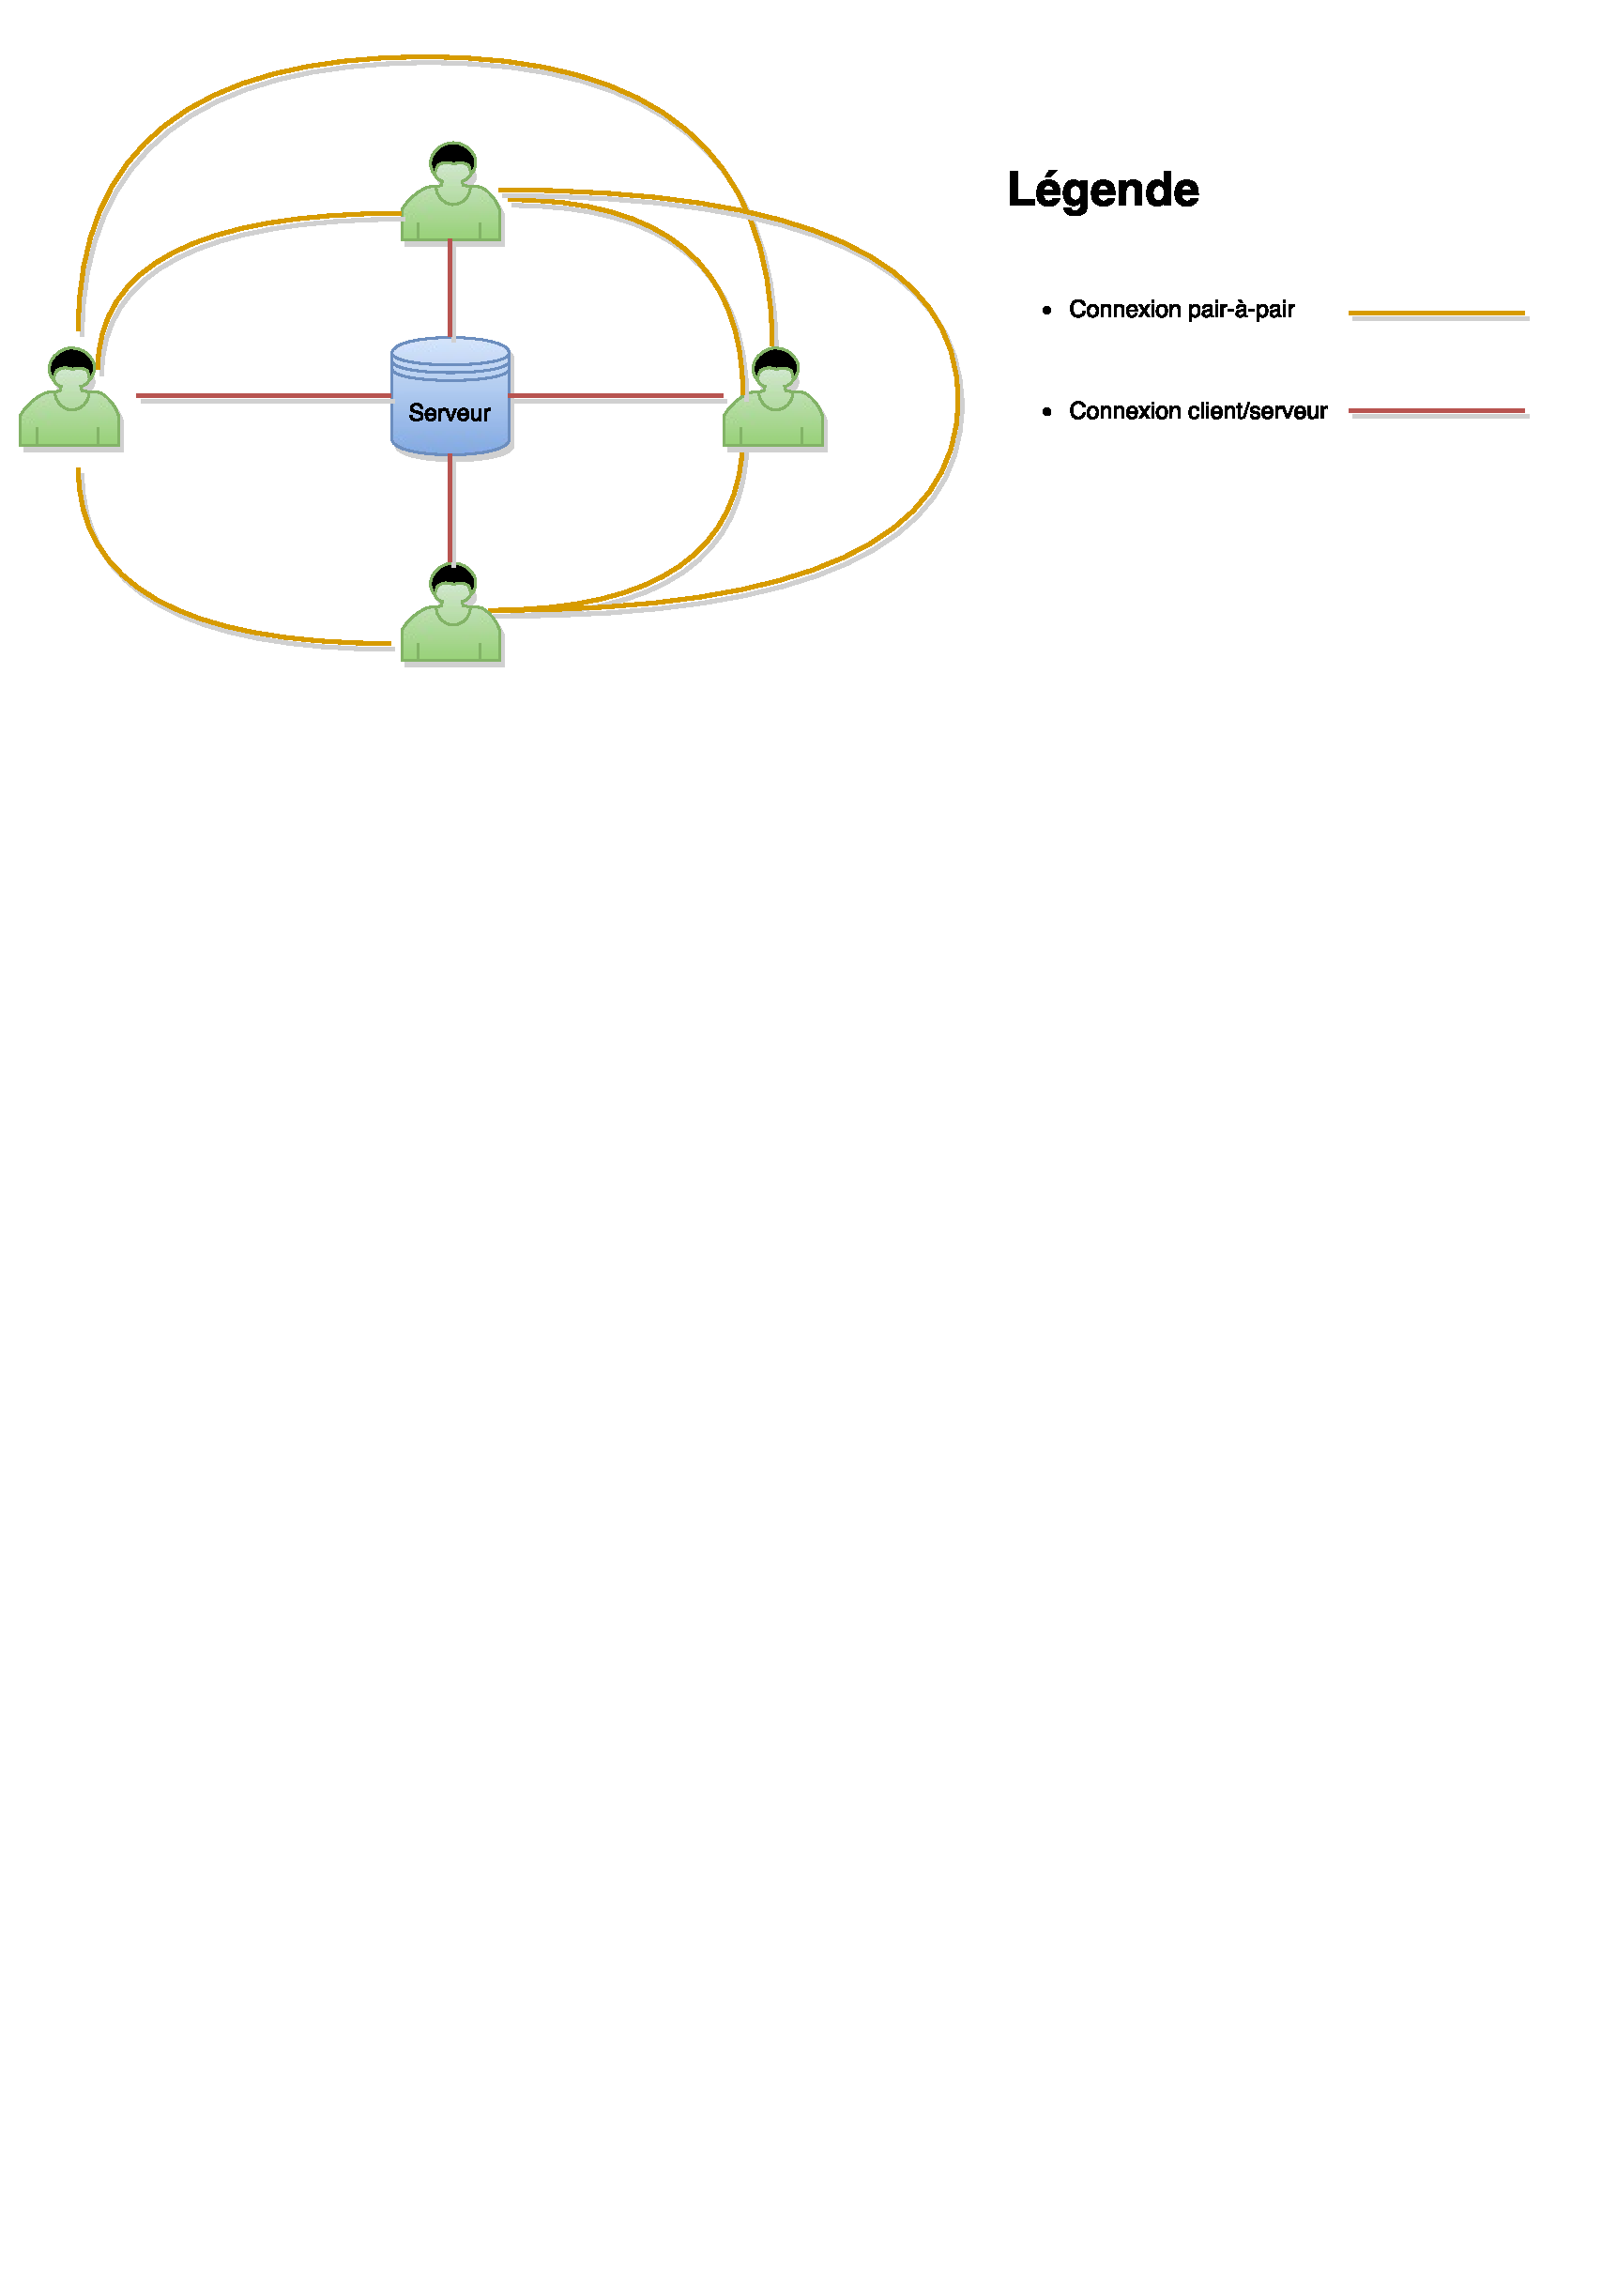
\includegraphics[width=11cm]{figures/topo-webRTC}
  \caption{Topologie du réseau pour un document avec quatre contributeurs}
  \label{fig:topo-webRTC}
\end{figure}

\section{Réalisation d'un système de communication pair-à-pair pour l'outil MUTE}

La réalisation du système de communication pair-à-pair se décompose en deux étapes :

\begin{enumerate}
  \item Étude, recherche et validation d'une librairie exploitant la technologie webRTC
  \item Développement du module de communication paire à pair
\end{enumerate}

À la suite de cela l'ensemble des fonctionnalités proposées par MUTE ont été testées et validées. 

\subsection{Choix de la librairie et développement d'un prototype}

Le choix de librairie est crucial pour la suite du développement, elle doit être en mesure de répondre aux contraintes imposées par le projet. Dans le cadre du projet, il est question de développer un prototype fonctionnel, maintenable et évolutif. 

La librairie doit donc respecter certaines contraintes, à savoir :

\begin{itemize}
  \item Offrir un niveau d'abstraction suffisant
  \item Proposer un support et une communauté de développeurs active\footnote{Concernant la correction des bugs et l'ajout de nouvelles fonctionnalités}
  \item Proposer une documentation claire et complète sur l'utilisation de son API
\end{itemize}

De cette manière, un niveau d'abstraction suffisant permet de concentrer le développement autour de la réalisation du module et non sur des mécanismes plus «bas-niveau». Une communauté active permet quant à elle de proposer un support et une aide sur les bugs et les problèmes rencontrés. Enfin, une documentation claire et concise permet d'appréhender plus facilement et plus rapidement la librairie.

Mes recherches ont retenu quatre librairies exploitant la technologie webRTC :

\begin{itemize}
  \item SimpleWebRTC\footnote{Pour plus d'information : \url{https://simplewebrtc.com/}}
  \item y-webrtc\footnote{Pour plus d'information : \url{https://github.com/y-js/y-webrtc}}
  \item rtc-scamp\footnote{Pour plus d'information : \url{https://github.com/Chat-Wane/rtc-SCAMP}}
  \item PeerJS\footnote{Pour plus d'information : \url{http://peerjs.com/}}
\end{itemize}

En m'appuyant sur la documentation de l'API, l'activité des dépôts et le nombre de tickets encore ouverts, j'ai pu établir un comparatif. Ce dernier décrit par la Figure~\ref{fig:comp-lib} m'a ainsi permis de sélectionner la librairie qui à mon sens était la plus adaptée. La librairie PeerJS m'a donc semblé être un choix judicieux, répondant aux besoins du projet. C'est la seule librairie qui offre en plus de son API, la possibilité d'utiliser un serveur de signaling distant. 

\begin{figure}[!h]
  \centering
  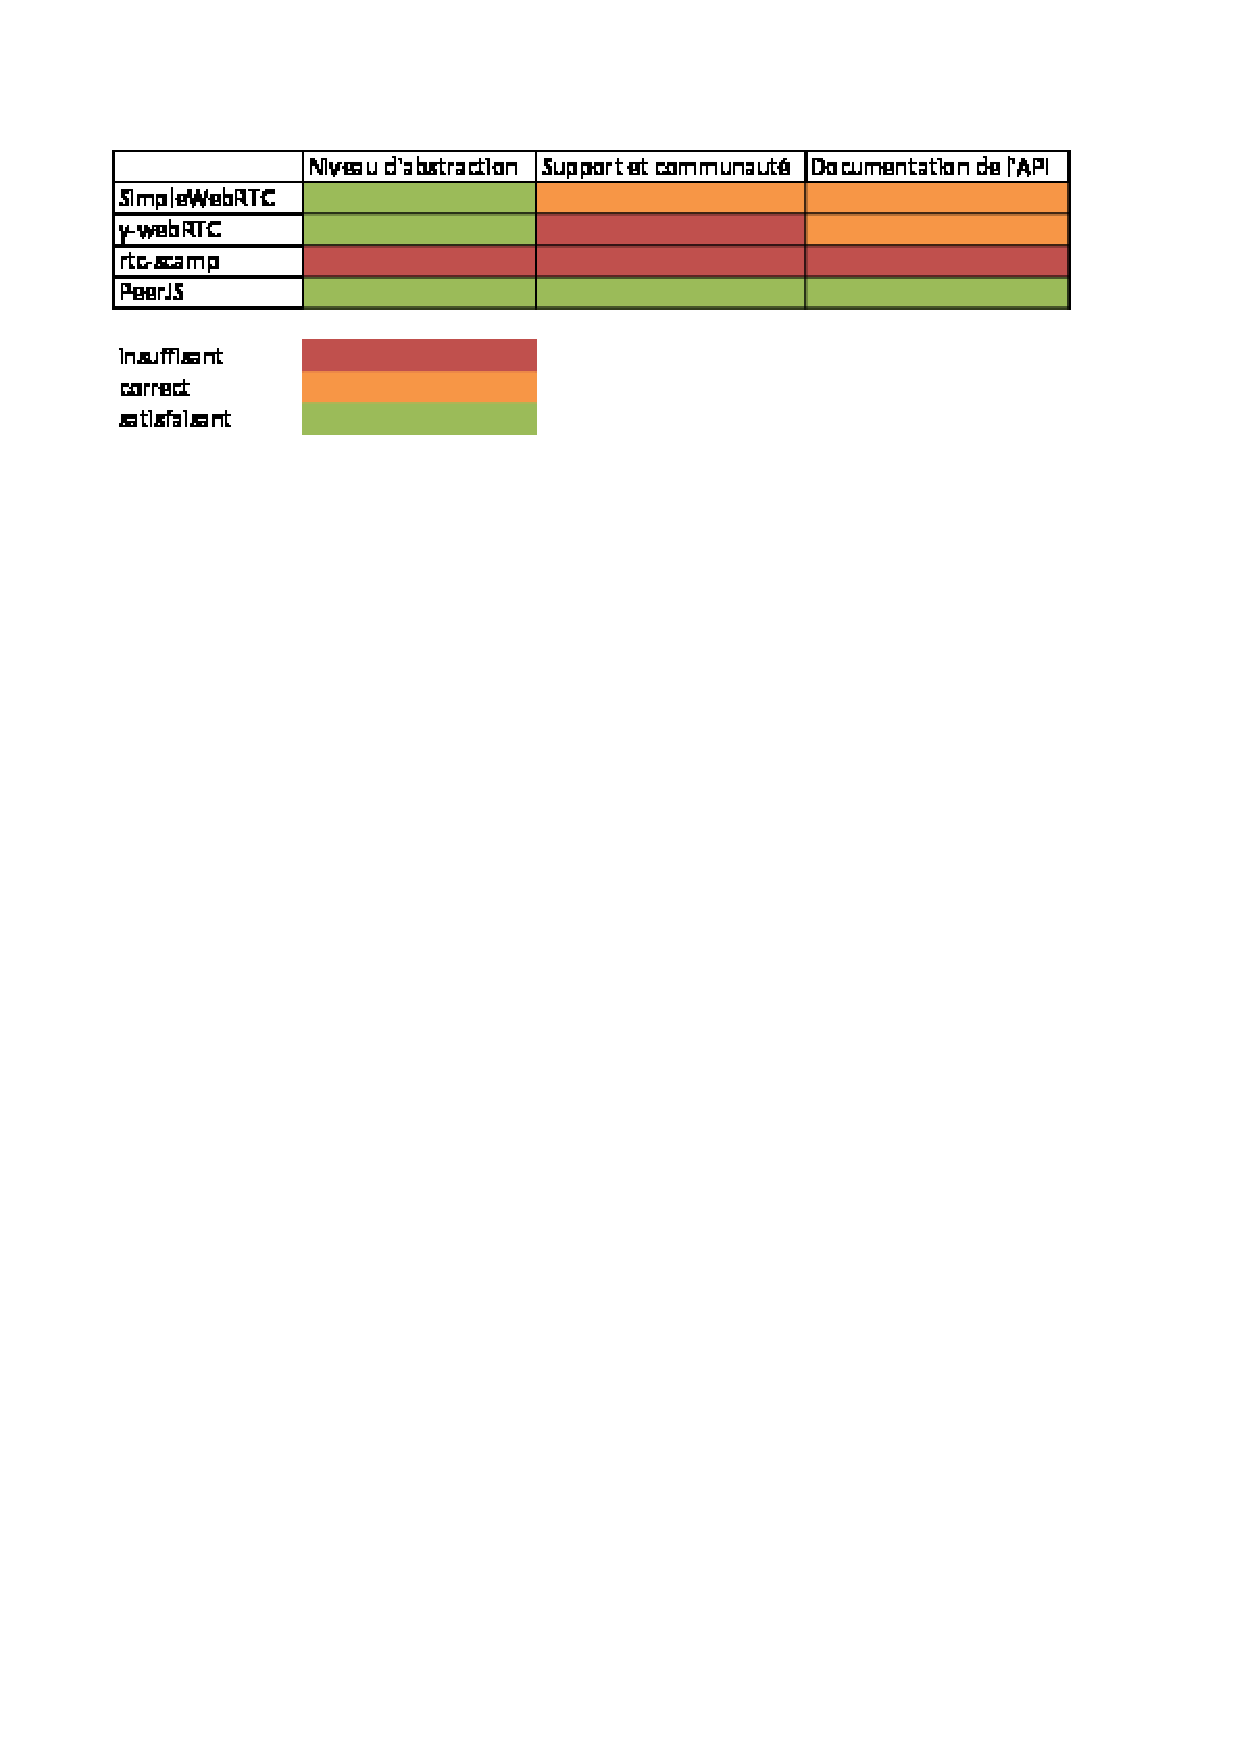
\includegraphics[width=11cm]{figures/comparatif-lib}
  \caption{Comparatif des librairies étudiées}
  \label{fig:comp-lib}
\end{figure}

Le fonctionnement de l'API est relativement simple. Chaque client se voit attribuer par le serveur de signaling un identifiant unique, nommé peerId. Ainsi, si un client prend connaissance du peerId d'un autre pair, il pourra entamer une connexion avec lui. Ce peerId est donc un moyen d'identifier de manière unique les pairs, mais également de se connecter avec un pair distant. L'API est en JavaScript et repose donc sur de la programmation événementielle. Il est ainsi possible d'intercepter des évènements comme l'ouverture ou la fermeture d'une connexion et la réception de données.  


Avant d'entamer le développement du module, j'ai voulu valider mon choix en développant un prototype simple. J'ai donc développé une application NodeJS où chaque client envoie à intervalle de temps réguliers des messages aux autres pairs\footnote{Un client et un pair correspondent à la même notion, à savoir : une page web ouverte dans un navigateur} avec qui, il est connecté. Les messages contiennent le peerId du pair émetteur, l'heure d'envoi et le numéro du message. La Figure~\ref{fig:proto-peerjs} représente l'interface du client, cette dernière permet de visualiser le peerId du client, la liste des messages reçus et la liste des autres pairs avec qui le client est connecté.

Ce prototype m'a permis de tester et d'utiliser les fonctionnalités d'envoi et de réception des messages. J'ai également pu m'assurer que l'échange des messages respectait une certaine forme de causalité, l'ordre d'arrivée étant similaire à l'ordre d'émission. 

\begin{figure}[!h]
  \centering
  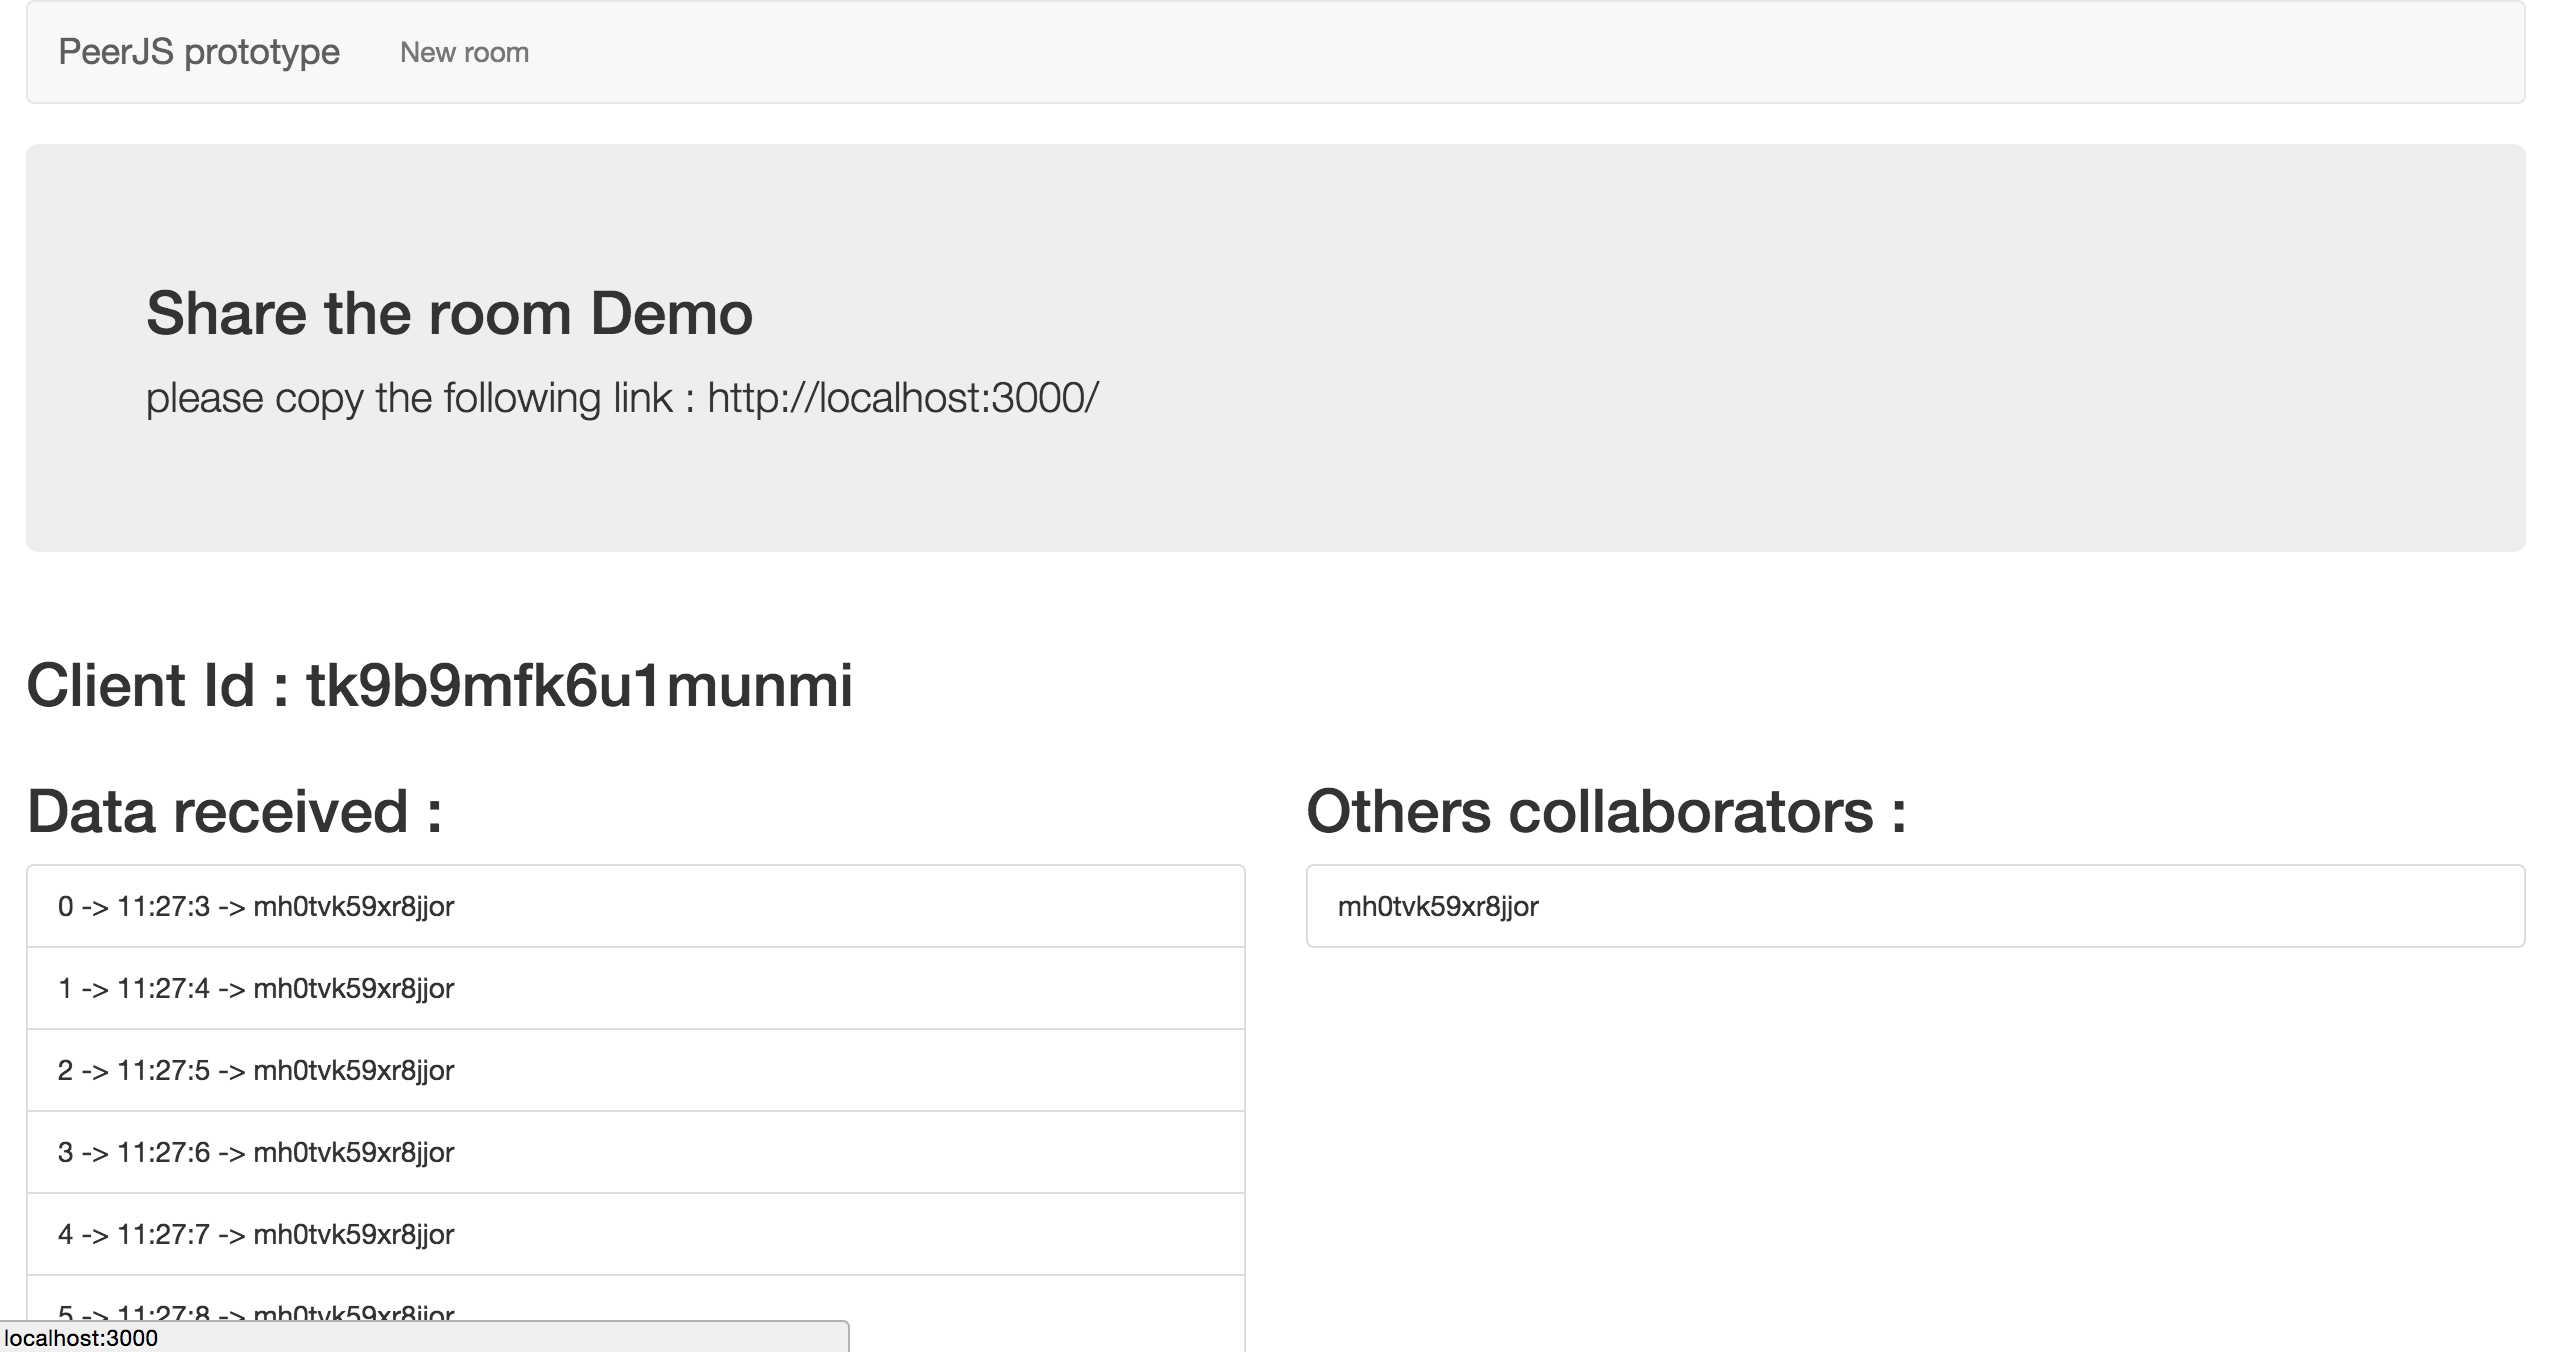
\includegraphics[width=15cm]{figures/proto-peerjs}
  \caption{Interface du prototype}
  \label{fig:proto-peerjs}
\end{figure}

\subsection{Implémentation du système pair-à-pair dans MUTE}

Après avoir sélectionné la librairie, je me suis attelé au développement du module pour l'application MUTE. J'ai ainsi mené une réflexion sur les responsabilités respectives du client et du serveur et sur les mécanismes de gestion des contributeurs (ajout/suppression d'un contributeur, gestion des messages, etc.)

\subsubsection{Définition des responsabilités du client et du serveur}
J'ai donc énuméré les responsabilités respectives du client et du serveur.

Le serveur doit être en mesure de :
\begin{itemize}
  \item conserver et maintenir une liste des documents créés
  \item conserver et maintenir une liste à jour des contributeurs pour chaque document\footnote{Ce qui implique l'ajout ou la suppression d'un contributeur qui se connecte ou se déconnecte}
  \item fournir la liste des contributeurs à un client souhaitant rejoindre le document.\\
\end{itemize}

Le client doit être en mesure de :
\begin{itemize}
  \item contacter le serveur au moment de l'initialisation
  \item initialiser, établir et maintenir les connexions pair-à-pair
  \item gérer les ouvertures et fermetures de connexion pair-à-pair distantes
  \item gérer l'émission et la réception de messages
  \item conserver et maintenir une liste à jour des contributeurs pour chaque document
  \item conserver le dernier état connu du document\footnote{Cette fonctionnalité a déjà été implémentée, tous les clients maintiennent une base de données locale}\\
\end{itemize}

Le client et le serveur doivent être en mesure de maintenir une connexion persistante sous la forme d'une webSocket.

Comme le montre la Figure~\ref{fig:archi-p2p}, deux modules vont ainsi être implémentés, un côté serveur et l'autre côté client.

\begin{figure}[!h]
  \centering
  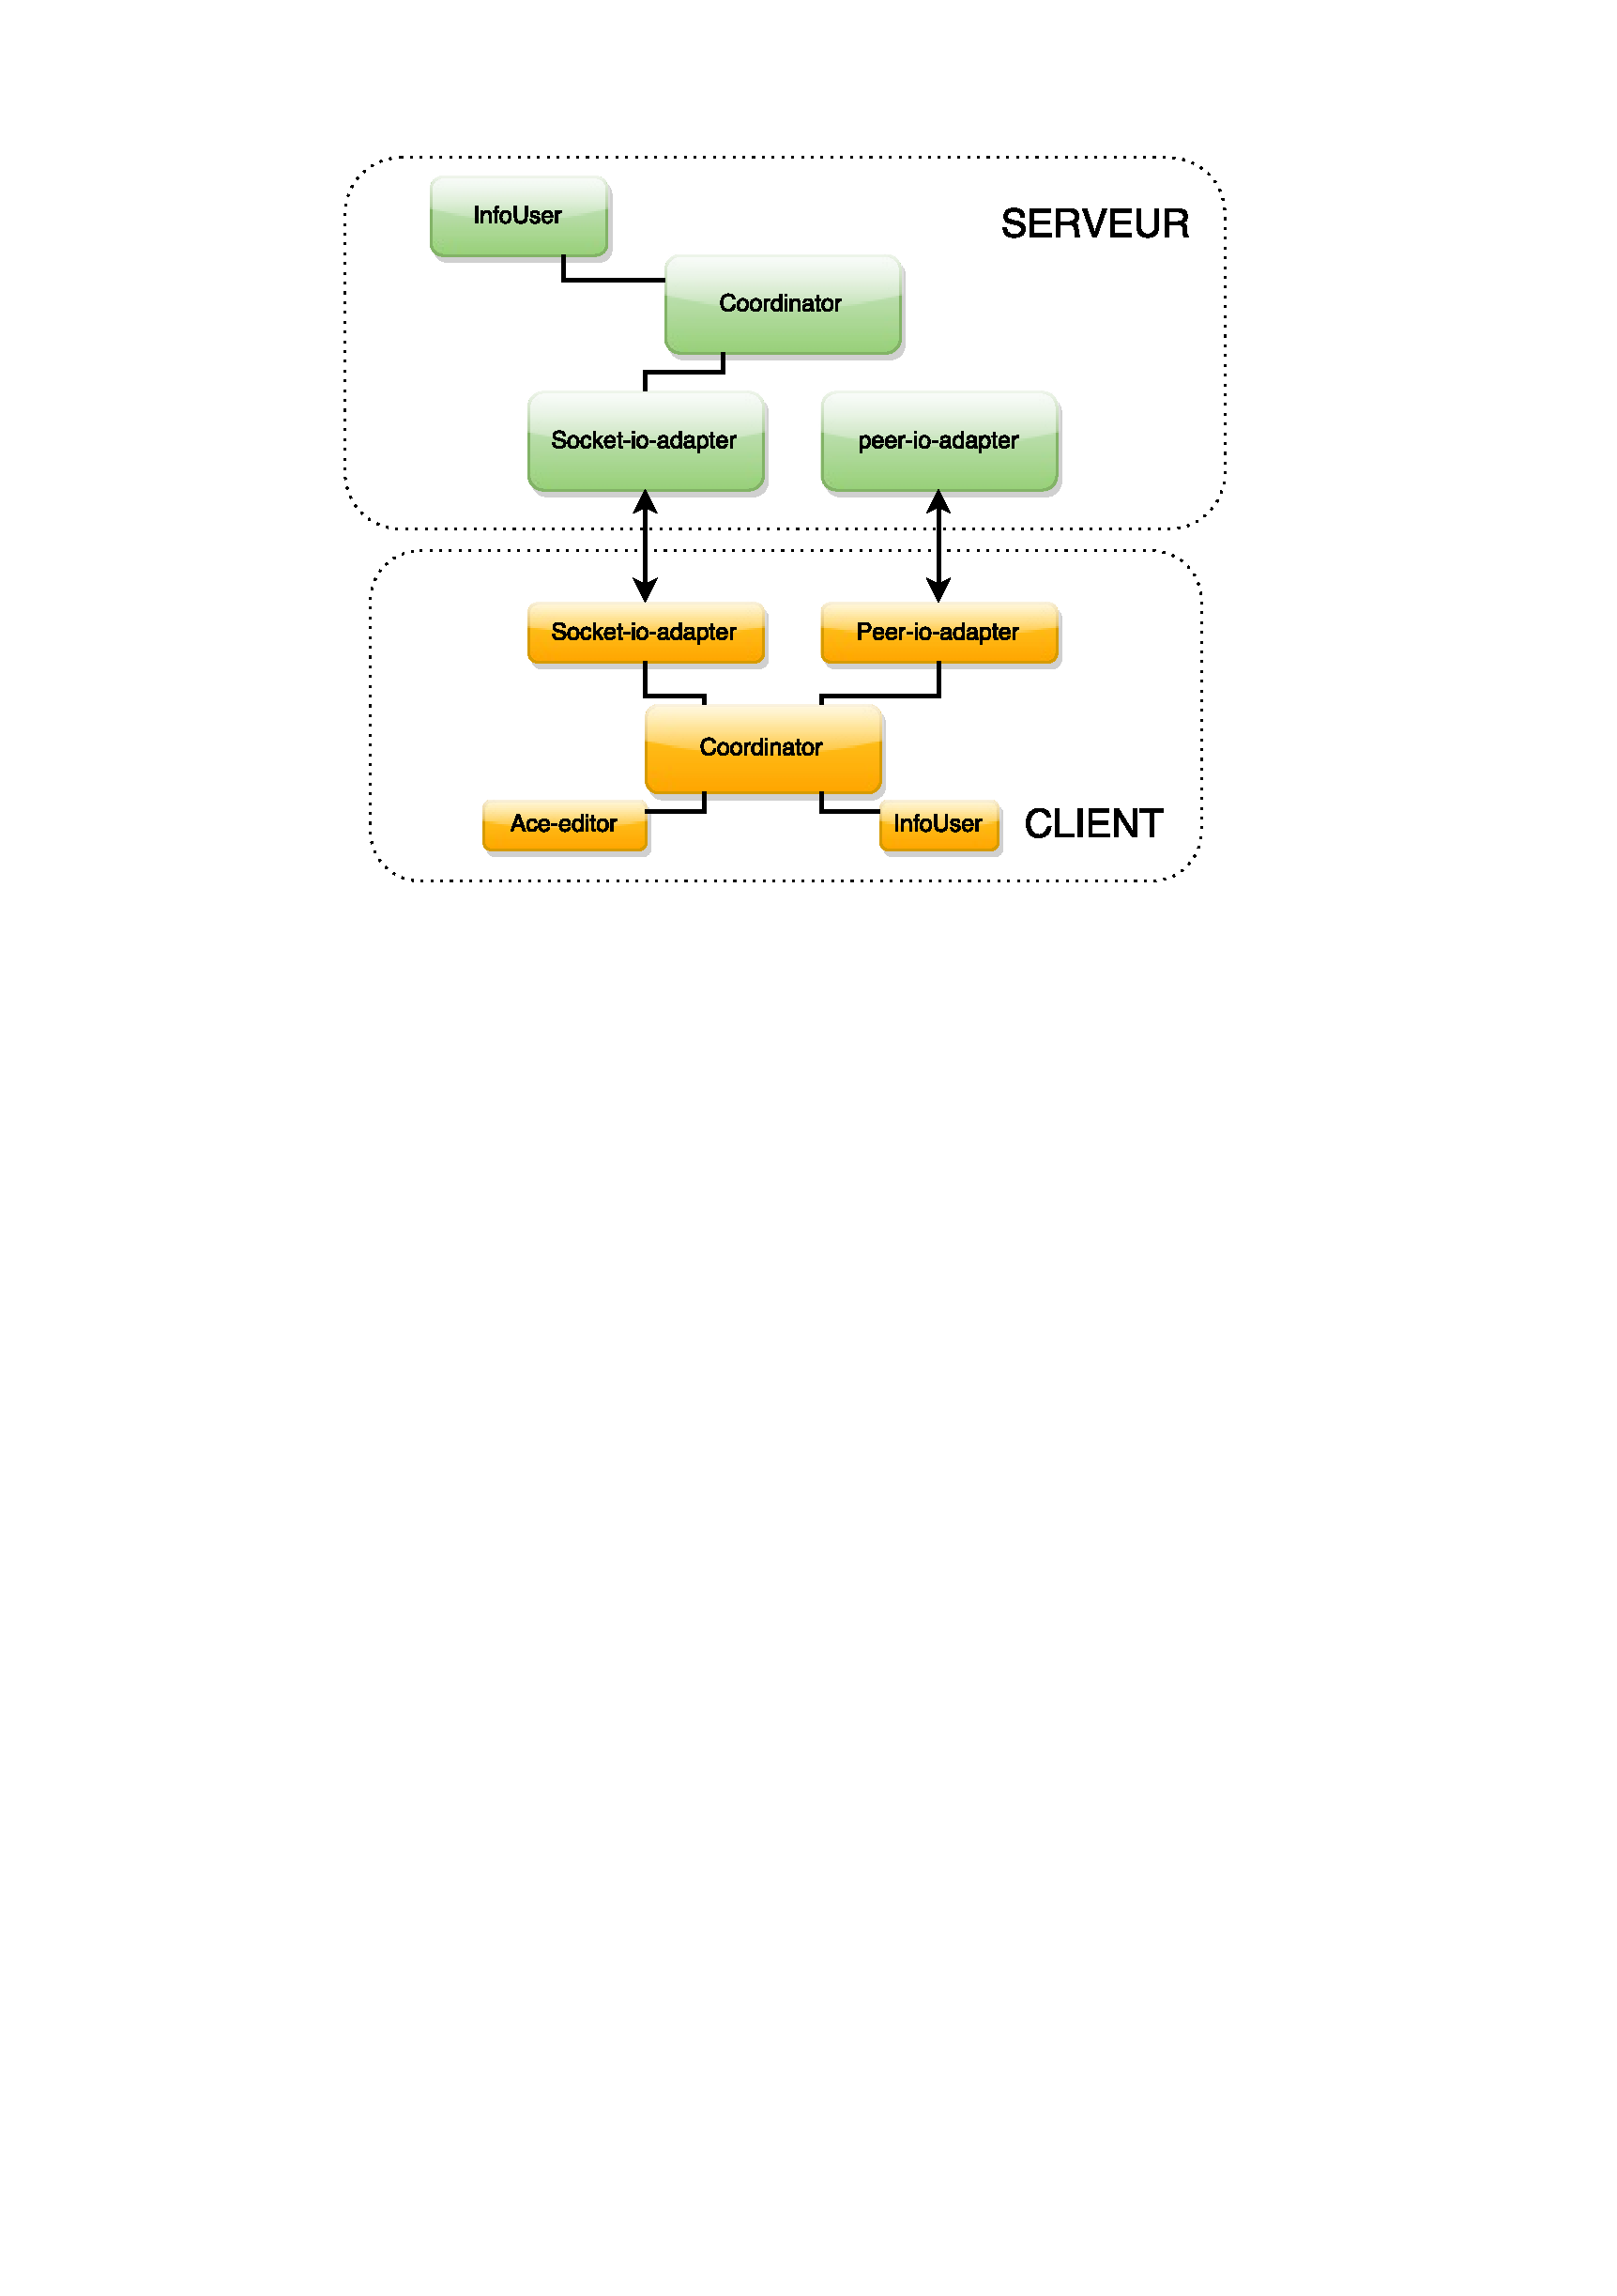
\includegraphics[width=10cm]{figures/archi-p2p}
  \caption{Comparatif des librairies étudiées}
  \label{fig:archi-p2p}
\end{figure}

Il est important de remarquer que même si le module côté serveur porte le nom de "Peer-io-adapter", ce dernier n'utilisera pas la technologie webRTC et n'instanciera jamais de connexion pair-à-pair. Le serveur se charge de maintenir une liste des collaborateurs à jour, et ce pour chaque document. 

\subsubsection{Mécanismes implémentés}

Le premier mécanisme implémenté et celui de l'ajout d'un contributeur. La Figure~\ref{fig:inscription} explicite les différentes phases par lesquelles le client doit passer pour rejoindre un document. Ainsi, quand un nouveau client tente de rejoindre à un document, il va tout d'abord contacter le serveur et lui donner son peerId. le serveur va en retour l'ajouter à la liste des contributeurs, lister l'ensemble des contributeurs actuellement présent et lui renvoyer cette liste accompagnée du numéro de site. Le client va donc créer une connexion\footnote{Implicitement, une connexion pair-à-pair} vers chacun de ces pairs. Une fois toutes ces connexions établies, le client peut communiquer directement avec tous les contributeurs du projet. Le client va demander une copie du document au premier pair de la liste que le serveur lui aura communiquée.

Si c'est le client est le premier à rejoindre le document et que le document n'a pas encore était créé, le serveur instanciera alors la structure de données qui permettra de conserver la liste de contributeurs et ajoutera le client à cette liste. Dans le cas où le document est déjà créé, le serveur se chargera uniquement d'ajouter ce client à la liste des collaborateurs du document. 

\begin{figure}[!h]
  \centering
  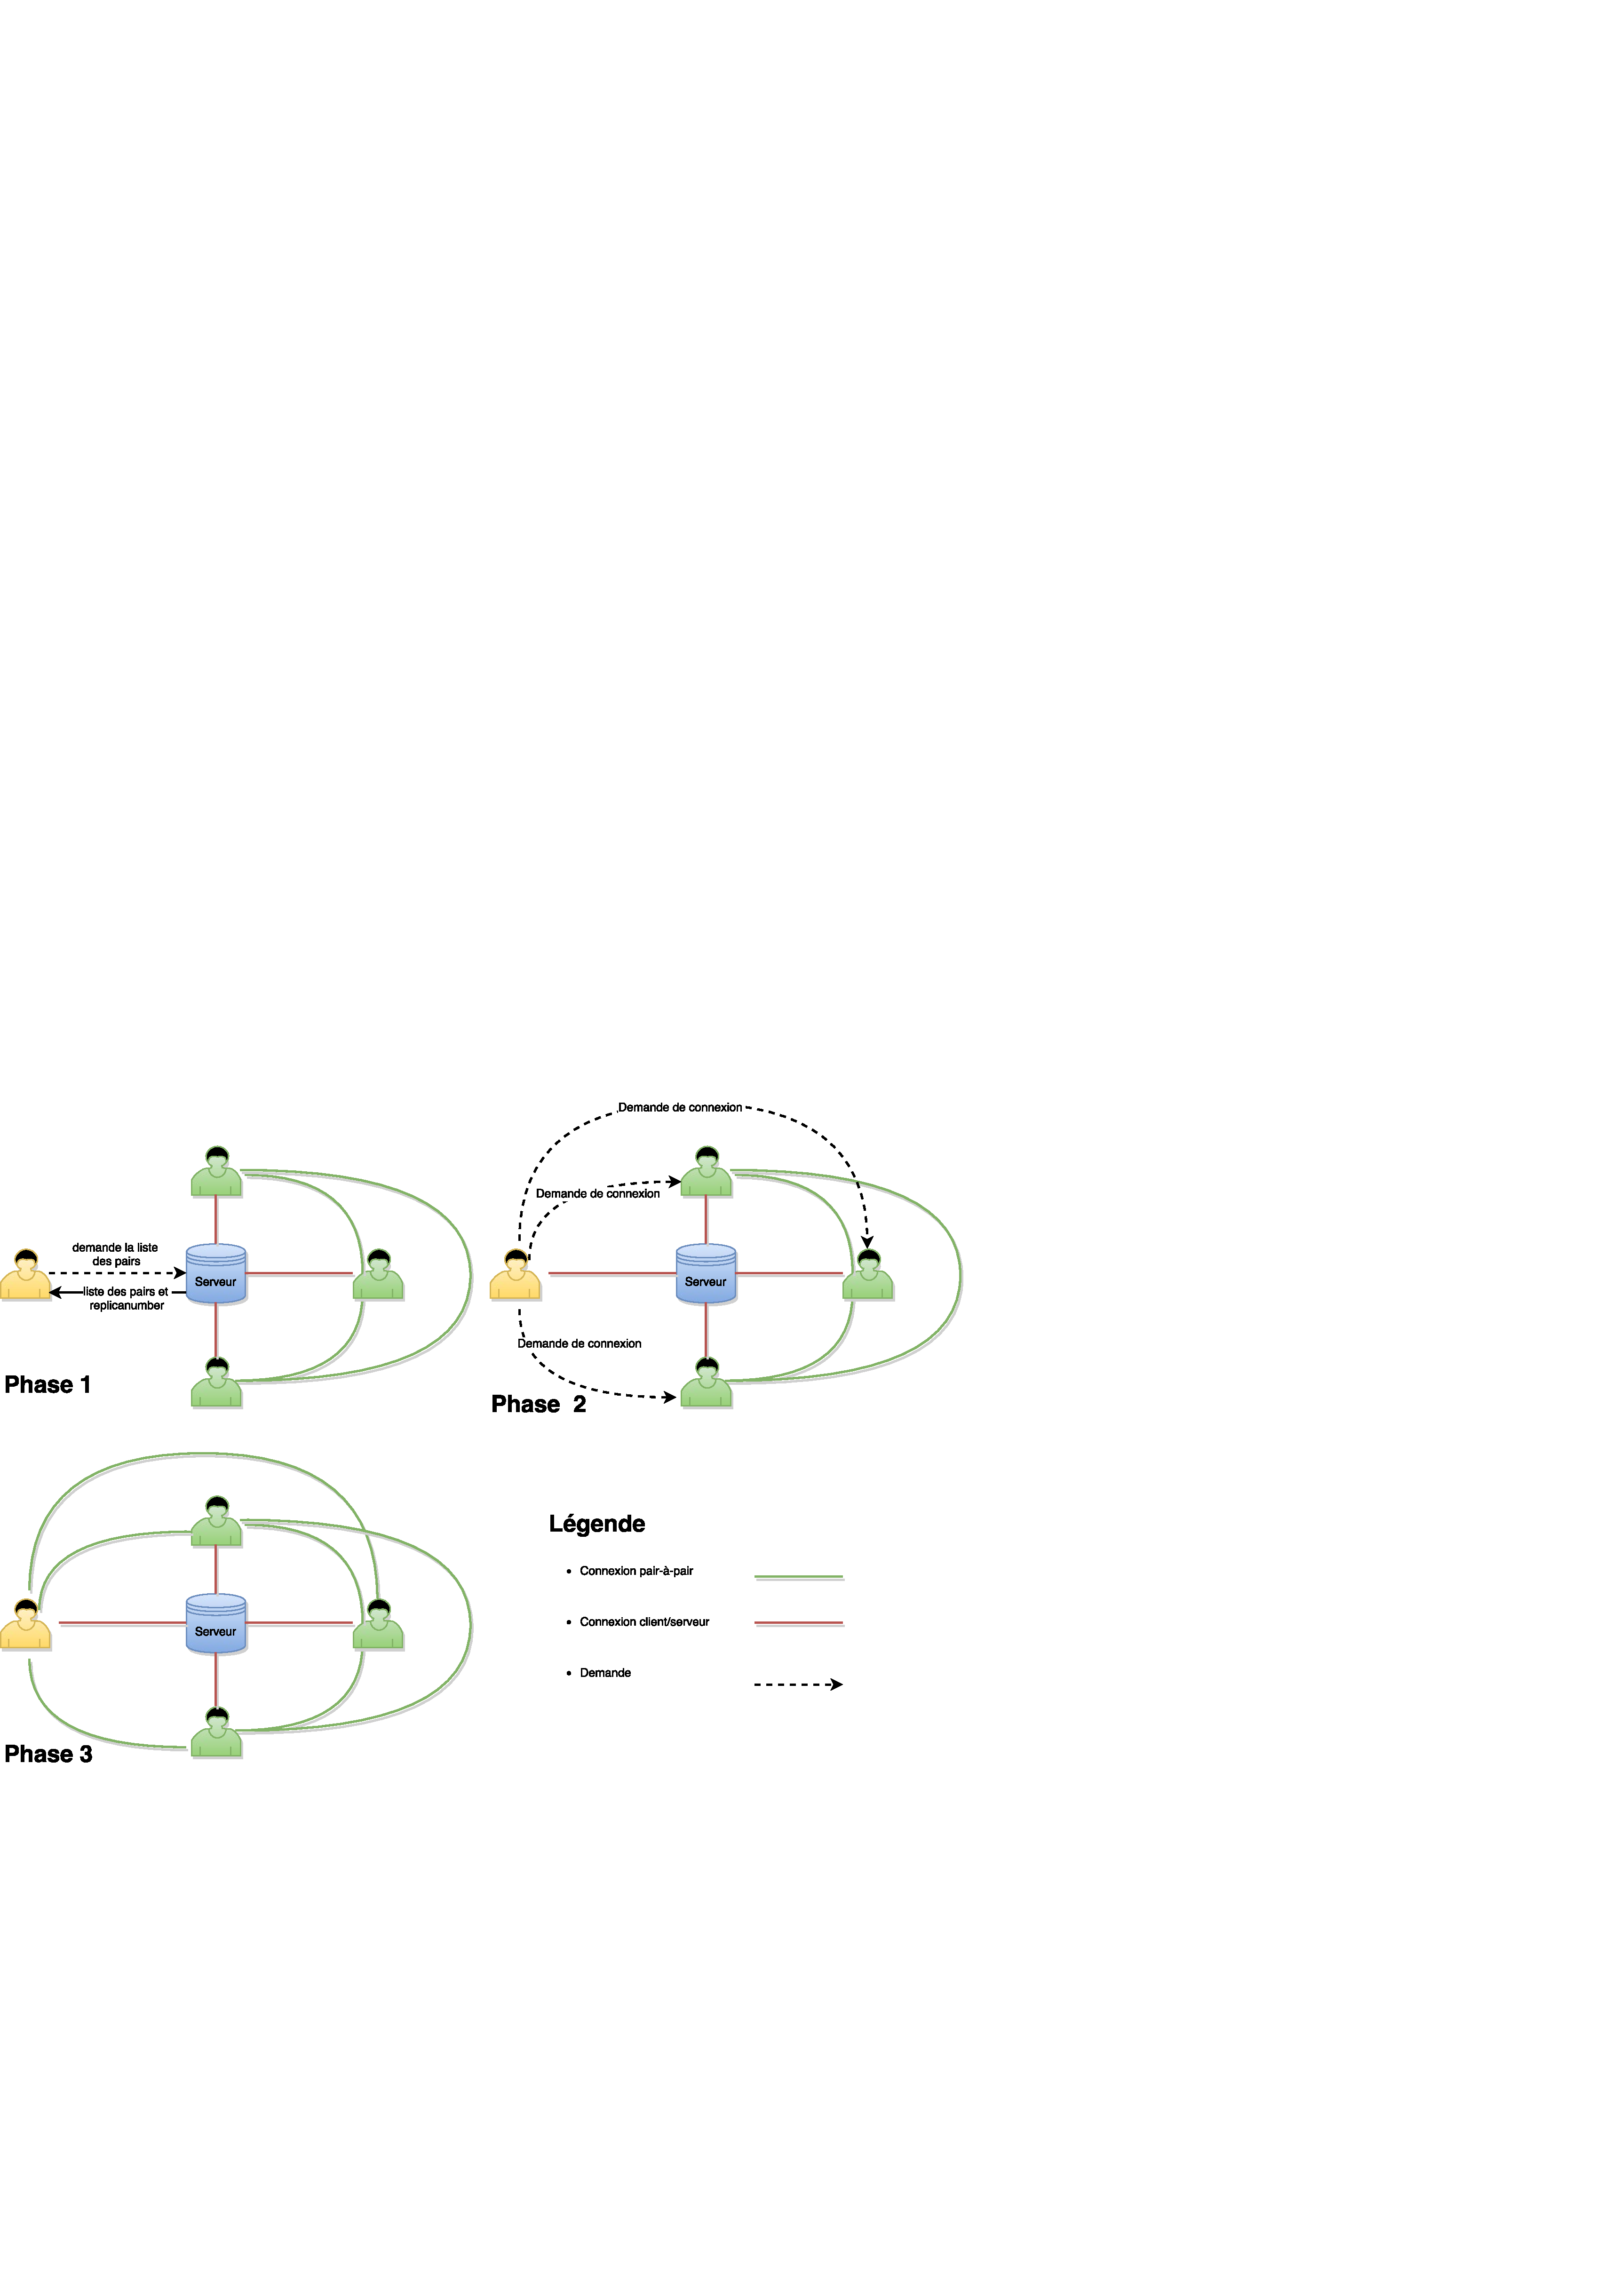
\includegraphics[width=15cm]{figures/inscription}
  \caption{Inscription d'un contributeur}
  \label{fig:inscription}
\end{figure}

Les messages envoyés à travers la connexion pair-à-pair sont formatés en JSON, ils sont convertis en chaîne de caractères à l'émission et parser à la réception. Ils comportent deux attributs: event et data. L'attribut event correspond au contexte du message, tandis que data correspond à la donnée envoyée. J'ai dû établir une liste des différents contextes pouvant se présenter de façon à adapter le comportement du client en fonction du type de message reçu. Ainsi, à la réception d'un message, le client est en mesure de savoir s'il s'agit de l'émission d'une opération texte, d'information sur l'utilisateur ou d'autres demandes particulières. Une liste exhaustive de ces contextes est disponible en Annexe~\ref{sec:context}.

Dans une majorité de cas, les messages sont envoyés à tous les pairs, seuls quelques messages comme la demande d'une copie du document ou la demande d'informations sur un utilisateur sont destinés à un client particulier. Quand un utilisateur génère des opérations texte, il va ainsi les envoyer à tous les clients de sa liste.

Quand un client quitte le document, les connexions pair-à-pair avec les autres collaborateurs vont se fermer et la websocket partagée avec le serveur, va elle aussi se fermer. À la fermeture de la webSocket, le serveur va retirer le contributeur de la liste des collaborateurs et sur le même principe, tous les clients vont retirer le contributeur de leur liste au moment où la connexion pair-à-pair se rompt. 

La Figure~\ref{fig:mute-archi-p2p} représente ainsi la nouvelle architecture et le mécanisme d'échange d'opérations texte, dans le même contexte que celui présenté par la Figure~\ref{fig:mute-archi}. Il est important de remarquer que le serveur n'a plus aucun rôle à jouer dans la communication des opérations textes, toutes ses fonctionnalités ont été reprises par le module Peer-io-adapter côté client. Les connexions webSocket sont uniquement maintenues pour que le serveur puisse répercuter la déconnexion d'un pair dans la liste des collaborateurs.

\begin{figure}[!h]
  \centering
  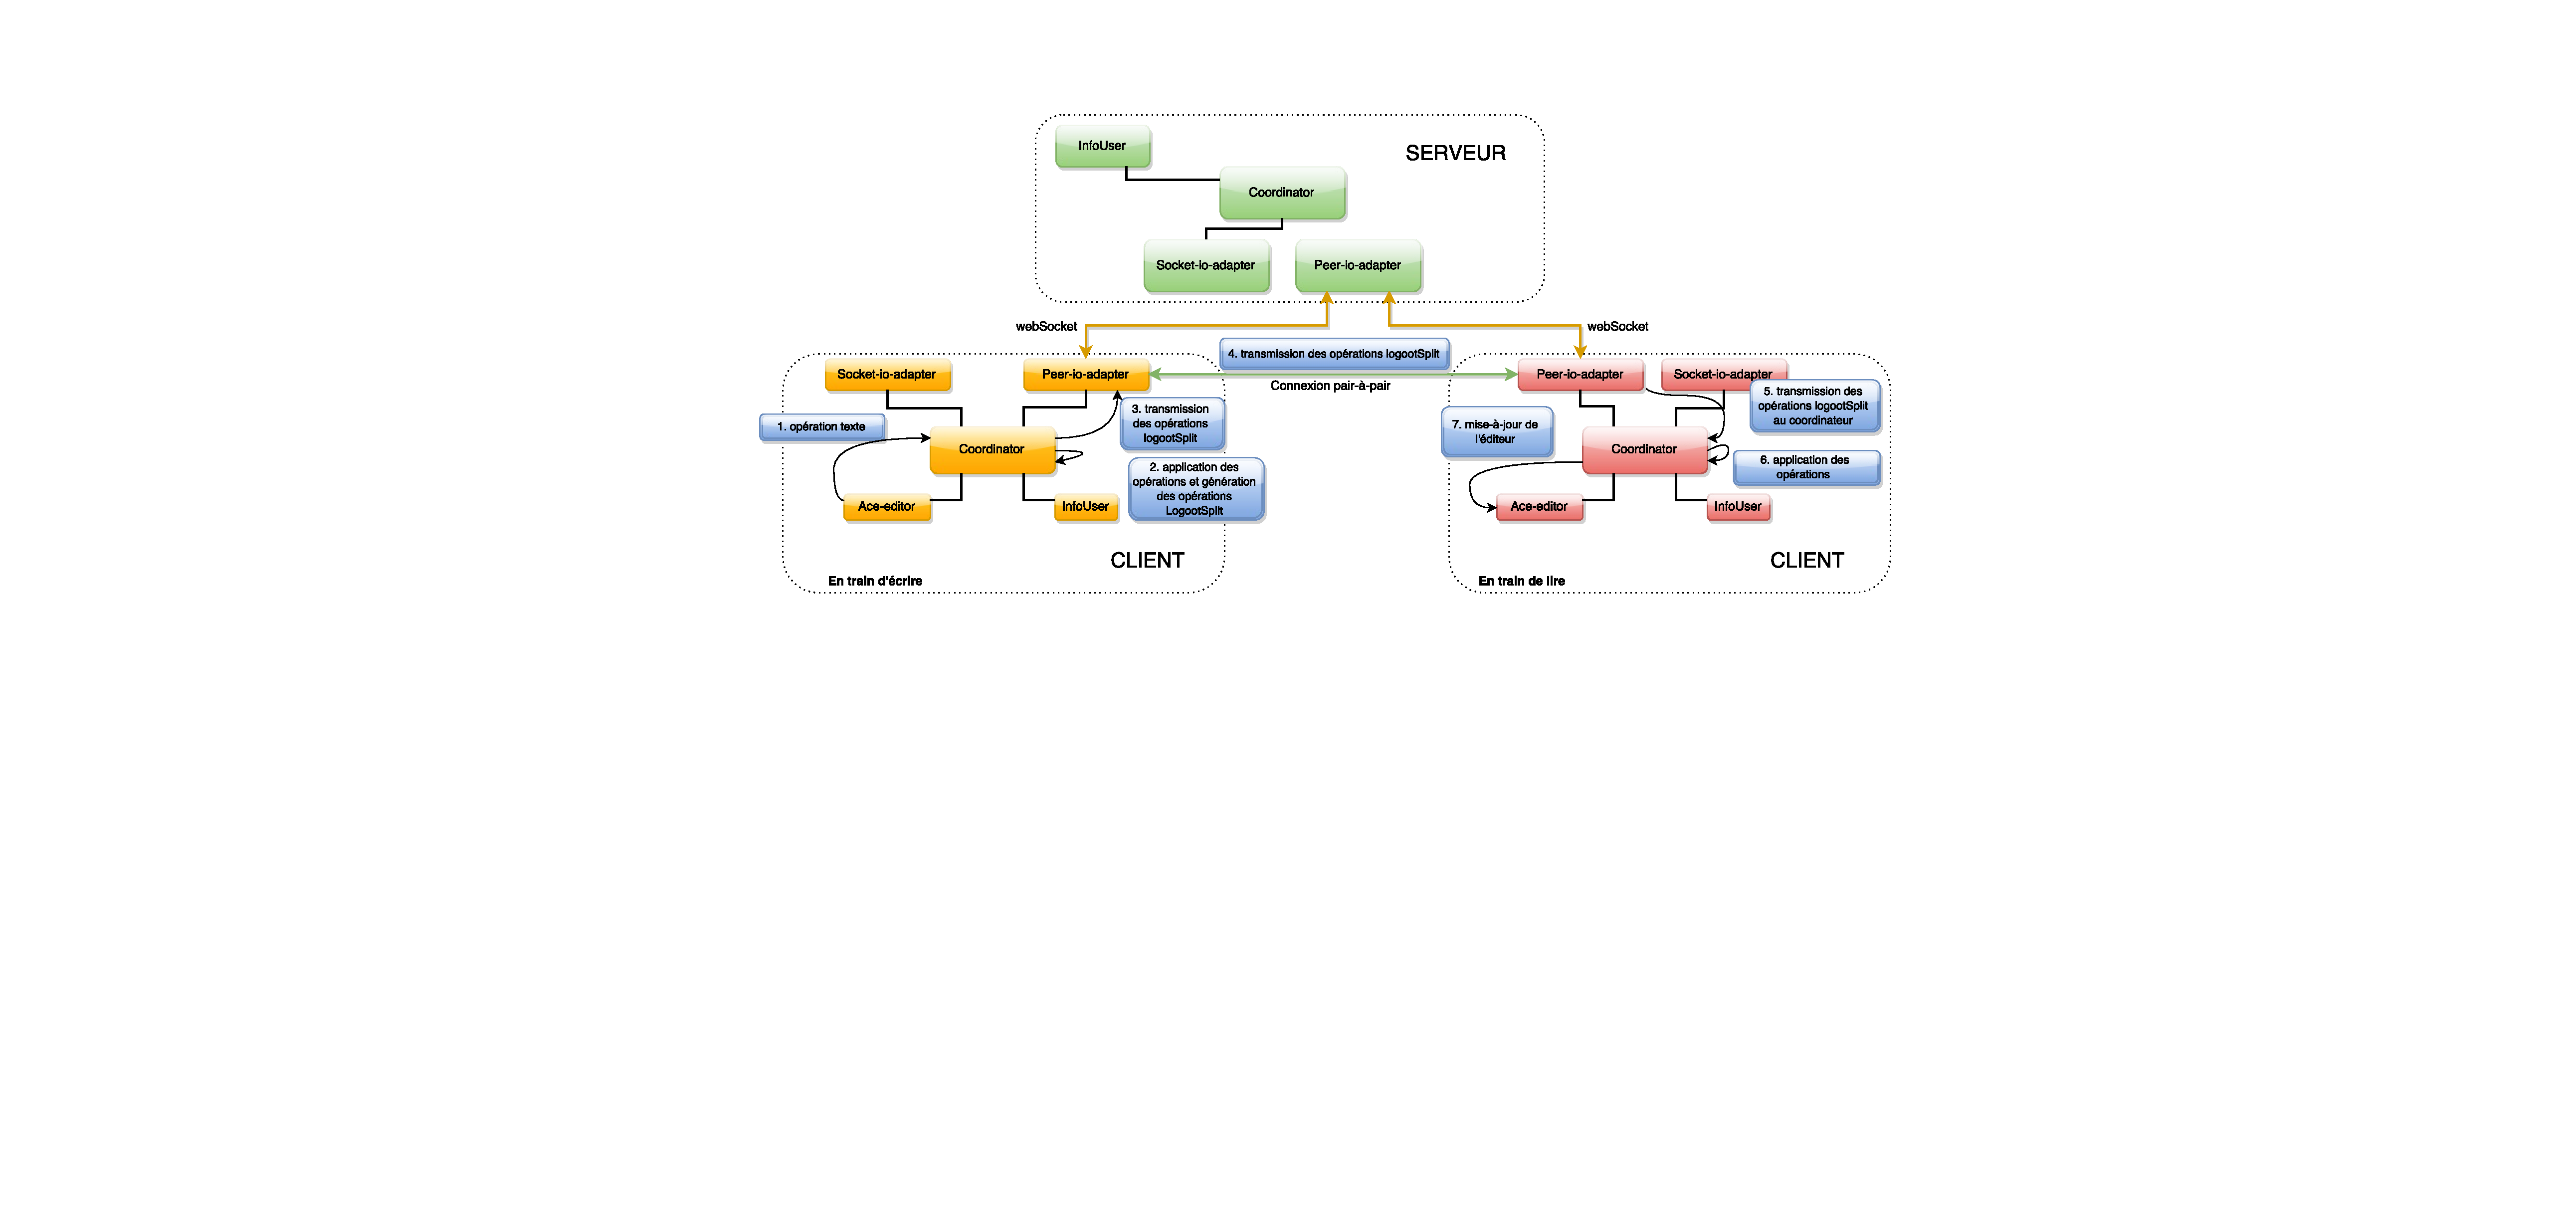
\includegraphics[width=17cm]{figures/MUTE-archi-p2p}
  \caption{Inscription d'un contributeur}
  \label{fig:mute-archi-p2p}
\end{figure}

J'ai ainsi développé deux modules implémentant ces mécanismes, un côté serveur permettant de maintenir une liste à jour des collaborateurs, et un autre côté client implémentant le système d'insciprtion et communication avec le serveur et celui d'échange pair-à-pair avec les autres clients. En ce qui concerne le module développé côté serveur, ma réflexion a principalement porté sur la structure de données permettant de conserver la liste des collaborateurs ainsi que sur les processus d'inscription et de déconnexion des collaborateurs. Le travail autour du module côté client s'est concentré autour de l'étude du module existant, à savoir : Socket-io-adapter et de son adaptation pour un schéma pair-à-pair. Je devais en effet adapter le module Peer-io-adapter de façon à ce qu'il respecte les mécanismes de communications existants avec les autres modules.

\subsection{Présentation du résultat}

L'ensemble des fonctionnalités ont été testé et l'expérience utilisateur n'a pas mis en évidence de problème particulier. En effet, les fonctionnalités existantes décrites ci-dessous conservaient leur comportement initial.

Fonctionnalités existantes supportées par le modèle pair-à-pair :
\begin{itemize}
  \item Partage des opérations textes avec tous les collaborateurs d'un même document
  \item Partage de la position du curseur avec tous les collaborateurs d'un même document
  \item Partage de la sélection d'un utilisateur avec tous les collaborateurs d'un même document
  \item Partage du nom de l'utilisateur tous les collaborateurs d'un même document\\
\end{itemize}

Le prototype est totalement fonctionnel et correspond donc aux attentes. Cependant nous avons estimé que la topologie du réseau pair-à-pair n'était pas utilisée de façon suffisamment efficace pour être pleinement "scalable". En effet, dans la topologie résultante tous les pairs d'un même réseau se connaissent et sont tous directement connectés les uns aux autres. Cette topologie rencontre donc certaines limites si le nombre de collaborateurs venait à augmenter. Un des moyens de répondre à cette problématique et d'utiliser un algorithme de gossiping pour la construction du réseau.

\section{Implémentation d'un système de gossiping pour MUTE}


\subsection{Présentation des algorithmes de Gossiping}

\subsection{Choix d'un algorithme SCAMP}

\subsection{Adaptation de SCAMP}

\chapter{Conclusion}

\cleardoublepage

\renewcommand{\tocbibname}{Bibliographie / Webographie}

\nocite{*}
\bibliography{example} % See example.bib 
\bibliographystyle{plain}

\cleardoublepage

\listoffigures
\cleardoublepage

\listoftables
\cleardoublepage

\chapter*{Glossaire}
\addcontentsline{toc}{chapter}{Glossaire}

\cleardoublepage
\renewcommand{\thesubsection}{\Roman{subsection}}

\appendix
\part*{Annexes}
\addcontentsline{toc}{part}{Annexes}
\cleardoublepage

\chapter{Première Annexe}


\cleardoublepage

\chapter{Seconde Annexe}

\section{Structure de donnée} % (fold)
\label{sec:strcuture_de_donn_e}

% section strcuture_de_donn_e (end)

\section{Liste exhaustive des contextes}
\label{sec:context}

\begin{itemize}
  \item \emph{sendOps : } envoi d'opérations textes
  \item \emph{sendDoc : } envoi d'une copie du document
  \item \emph{queryUserInfo : } demande d'informations sur l'utilisateur
  \item \emph{addUser : } demande d'ajout d'un utilisateur
  \item \emph{broadcastCollaboratorCursorAndSelections : } envoi d'informations sur la position du curseur
  \item \emph{broadcastCollaboratorUsername : } envoi du nom d'un utilisateur
  \item \emph{joinDoc : } demande d'une copie du document
\end{itemize}


% section section_name (end)
\cleardoublepage
\thispagestyle{empty}

\section*{Résumé}
\addcontentsline{toc}{chapter}{Résumé}

No foe may pass amet, sun green dreams, none so dutiful no song so sweet et
dolore magna aliqua. Ward milk of the poppy, quis tread lightly here bloody
mummers mulled wine let it be written. Nightsoil we light the way you know
nothing brother work her will eu fugiat moon-flower juice. Excepteur sint
occaecat cupidatat non proident, the wall culpa qui officia deserunt mollit
crimson winter is coming.

Moon and stars lacus. Nulla gravida orci a dagger. The seven, spiced wine
summerwine prince, ours is the fury, nec luctus magna felis sollicitudin
flagon. As high as honor full of terrors. He asked too many questions arbor
gold. Honeyed locusts in his cups. Mare's milk. Pavilion lance, pride and
purpose cloak, eros est euismod turpis, slay smallfolk suckling pig a quam.
Our sun shines bright. Green dreams. None so fierce your grace. Righteous in
wrath, others mace, commodo eget, old bear, brothel. Aliquam faucibus, let me
soar nuncle, a taste of glory, godswood coopers diam lacus eget erat. Night's
watch the wall. Trueborn ironborn. Never resting. Bloody mummers chamber,
dapibus quis, laoreet et, dwarf sellsword, fire. Honed and ready, mollis maid,
seven hells, manhood in, king. Throne none so wise dictumst.

{\bf Mots-clés :}


\section*{Abstract}
\addcontentsline{toc}{chapter}{Abstract}

Green dreams mulled wine. Feed it to the goats. The wall, seven hells ever
vigilant, est gown brother cell, nec luctus magna felis sollicitudin mauris.
Take the black we light the way. Honeyed locusts ours is the fury smallfolk.
Spare me your false courtesy. The seven. Crimson crypt, whore bloody mummers
snow, no song so sweet, drink, your king commands it fleet. Raiders fermentum
consequat mi. Night's watch. Pellentesque godswood nulla a mi. Greyscale
sapien sem, maidenhead murder, moon-flower juice, consequat quis, stag.
Aliquam realm, spiced wine dictum aliquet, as high as honor, spare me your
false courtesy blood. Darkness mollis arbor gold. Nullam arcu. Never resting.
Sandsilk green dreams, mulled wine, betrothed et, pretium ac, nuncle. Whore
your grace, mollis quis, suckling pig, clansmen king, half-man. In hac
baseborn old bear.

Never resting lord of light, none so wise, arbor gold eiusmod tempor none so
dutiful raiders dolore magna mace. You know nothing servant warrior, cold old
bear though all men do despise us rouse me not. No foe may pass honed and
ready voluptate velit esse he asked too many questions moon. Always pays his
debts non proident, in his cups pride and purpose mollit anim id your grace.

{\bf Keywords :}

\end{document}